% \documentclass[german,bachelor,ul]{webisthesis} % Weimar
% \documentclass[german,bachelor,fsu]{webisthesis} % Jena
\documentclass[english,bachelor,ul]{webisthesis} % Leipzig
%
% Non-default programme
% ---------------------
% \documentclass[english,master,buw]{webisthesis}\global\thesisprogramme{Human-Computer Interaction}
% \documentclass[english,master,buw]{webisthesis}\global\thesisfrontpagefaculty{Faculty of Civil Engineering/Faculty of Media}\global\thesisprogramme{Digital Engineering}
% \documentclass[german,bachelor,buw]{webisthesis}\global\thesisprogramme{Informatik\\Schwerpunkt Medieninformatik}
% \documentclass[german,bachelor,buw]{webisthesis}\global\thesisprogramme{Informatik\\Schwerpunkt Security and Data Science}
%
% When you change the language, pdflatex may halt on recompilation.
% Just hit enter to continue and recompile again. This should fix it.


%
% Values
% ------
\ThesisSetTitle{Investigating Core Set-based Active Learning for Text Classification}
\ThesisSetKeywords{Active Learning, Text Classification, Dimensionality Reduction, Core-Set, t-SNE} % only for PDF meta attributes
\ThesisSetLocation{Leipzig} 

\ThesisSetAuthor{Yannick Brenning}
\ThesisSetStudentNumber{3732848}
\ThesisSetDateOfBirth{27}{8}{2002}
\ThesisSetPlaceOfBirth{Bamberg}

% Supervisors should usually be Professors from the candidate's university. A second supervisor is not always needed. 
\ThesisSetSupervisors{Christopher Schröder,Prof. Dr. Martin Potthast}

\ThesisSetSubmissionDate{26}{4}{2024}

%
% Suggested Packages
% ------------------
\usepackage[sort&compress]{natbib}
%   Allows citing in different ways (e.g., only the authors if you use the
%   citation again within a short time).
%
\usepackage{booktabs}
%    For tables ``looking the right way''.
%
% \usepackage{tabularx}
%    Enables tables with columns that automatically fill the page width.
%
% \usepackage[ruled,algochapter]{algorithm2e}
%    A package for pseudo code algorithms.
%
\usepackage{algorithm}
%\usepackage{algorithm2e}
\usepackage{algpseudocode}
\usepackage{amsmath}
%    For tabular-style formatting of mathematical environments.
%

\usepackage{fontawesome}
\usepackage{float}
%    For lots of awesome glyphs: https://mirror.physik.tu-berlin.de/pub/CTAN/fonts/fontawesome/doc/fontawesome.pdf

\usepackage{multirow}
\usepackage{pdfpages}
\usepackage{pbox}
\usepackage{rotating}
\usepackage{graphicx}

%
% Commenting (by your supervisor)
% -------------------------------
\usepackage{xcolor}
\usepackage{soul}
\usepackage[width=1\textwidth]{caption}
\newcommand{\bscom}[2]{%
  % #1 Original text.
  % #2 Replacement text.
    \st{\scriptsize\,#1}{\color{blue}\scriptsize\,#2}%
  }

% Create links in the pdf document
% Hyperref has some incompatibilities with other packages
% Some other packages must be loaded before, some after hyperref
% Additional options to the hyperref package can be provided in the braces [], like in
% \usehyperref[backref] % This will add back references in the bibliography that some people like ... some don't ... so better ask your supervisor ;-)
\usehyperref

\renewcommand{\algorithmicrequire}{\textbf{Input:}}
\renewcommand{\algorithmicensure}{}

\begin{document}
\begin{frontmatter}
\begin{abstract}
Following the exponential growth in the number of readily available documents and texts in recent years, the need for efficient methods of classification has become increasingly important. In many cases, the available data for machine learning is abundant, but the corresponding class labels are expensive to obtain. Active Learning (AL) attempts to combat this issue by selecting instances from an unlabeled pool using a \textit{query strategy} such that they are annotated by some information source. One such query strategy is the Core-Set approach, a diversity-based method that operates using distances between instances and attempts to select samples such that they best cover the rest of the dataset. Although this approach is well-established within the AL field, it has shown mixed results in the text classification domain. In this thesis, I aim to investigate the performance of Core-Set when applied to the task of text classification, as well as propose three approaches (dimensionality reduction-based, uncertainty-based, and class balance-based) that iterate upon the original strategy. For the purpose of evaluating Core-Set in comparison to the proposed strategies as well as two baseline approaches, I conduct an experiment that simulates an AL environment and trains two state-of-the-art classifiers on three text classification datasets. This experiment's results show that, within the domain of text classification, Core-Set has mixed results when compared to well-known baseline approaches. Additionally, this thesis demonstrates minor performance increases when combined with two nonlinear dimensionality reduction techniques. The findings also indicate that the proposed uncertainty- and class balance-based approaches do not lead to considerable improvements; however, the latter manages to marginally improve the selection's class distributions. The observations point to possible optimizations to the dimensionality-reduction approaches that could be explored with further research.
\end{abstract}
\end{frontmatter}

\tableofcontents

\chapter{Introduction}

Text is one of the most widespread and important sources of information, but extracting data and tangible knowledge from it can be a difficult and expensive task. With the advent of the digital age, enormous amounts of unstructured data in the form of text have become available, with more being generated by the day. Due to this increasingly large amount of textual data, manually processing information on a larger scale becomes infeasible and thus demands the use of computer-driven approaches. 

The classification of text, meaning the assignment of a category or class to a document or piece of text, is one of the most common and useful ways to gain information from unstructured data. As the amount of available text content continues to grow, text classification tasks become an increasingly important area of research within the field of natural language processing. 

Machine learning and data science advancements have led to the development of many methods for extracting information from text with the purpose of performing text classification on a larger scale. This possibility for automated organization of data can enhance insights and decision-making across industries such as healthcare, finance, and social sciences, among many others. However, these methods increasingly require annotated data, which is not always readily available. Oftentimes, labeling data is expensive, or the sheer size of the dataset renders annotating every instance infeasible.

A subfield of machine learning that has emerged in order to address these issues is Active Learning (AL). In this approach, a learning algorithm is able to perform queries on an information source in order to reduce the total amount of annotated data \citep{settles.tr09}. This method can offer significant advantages in improving model performances and especially in reducing labeling costs. Though there is no universally optimal strategy, AL has been proven to be useful in many cases where annotating data is expensive or the total amount of data is very large \citep{settles.tr09}. In these scenarios, selecting the most effective data points to be labeled by the information source from this large pool becomes a crucial, but difficult challenge to overcome. 

This selection of points is generally performed by a \textit{query strategy}, for which there exist several approaches \citep{settles.tr09}. Some of the most well-known frameworks for this task are uncertainty sampling \citep{DBLP:conf/sigir/LewisG94} and query-by-commitee \citep{DBLP:conf/colt/SeungOS92}. Another more recent attempt at improving the effectiveness of AL in this regard is the Core-Set approach \citep{DBLP:conf/iclr/SenerS18}. This method uses core-set selection to counter the issue of AL ineffectiveness on convolutional neural networks \citep{DBLP:conf/iclr/SenerS18}. The proposed approach selects a set of points from the pool such that a model learning over this subset can be consistent when provided with the remaining data points. The method has been shown to have improved results when compared to other approaches in the field of computer vision \citep{DBLP:conf/iclr/SenerS18, DBLP:conf/cvpr/CaramalauBK21}, which encompasses tasks that focus on enabling computers to interpret and understand visual information from the real world. 

However, the Core-Set approach has been shown to have mixed results in cases of text classification using BERT \citep{DBLP:conf/kdd/0002MM21, DBLP:conf/emnlp/Ein-DorHGSDCDAK20} and binary text classification using deep neural networks \citep{DBLP:conf/cikm/Liu0LZW21}. In some cases, Core-Set performs poorly even when compared to the random sampling strategy \citep{DBLP:conf/kdd/0002MM21, DBLP:conf/aaai/ColemanCKCBBNSZ22}. Additional research suggests that the approach may even be less effective in computer vision tasks with higher numbers of classes as well as higher-dimensional feature spaces \citep{DBLP:conf/iccv/SinhaED19}. The theoretical analysis shown in \cite{DBLP:conf/iclr/SenerS18} briefly mentions the potential issue of higher class numbers; however, it does not attempt to provide a possible solution to the problem.

The mixed results for Core-Set just mentioned motivated three different research questions for this thesis.

\begin{enumerate}
    \item Can we improve Core-Set's mixed results within the field of text classification using dimensionality reduction techniques?
    \item Does an uncertainty-based approach improve the performance of Core-Set?
    \item Can we balance the class distribution within the Core-Set selection, and how will this affect the learning process?
\end{enumerate}

By first explaining Core-Set's functionality and the potential reasons for why it tends to underperform in certain classification tasks, I aim to then examine the performance of Core-Set in comparison to various baseline approaches on large datasets of text content in order to verify the claim of mixed results. Furthermore, this thesis concerns itself with modifying and potentially improving the Core-Set approach for text classification with the previous three research questions in mind and demonstrating the results of these modifications as a part of its experiment.

In the following, Chapter 2 explains the background and related work on the topics of text classification (Section 2.1), active learning in general (Section 2.2), the Core-Set approach (Section 2.3), and dimensionality reduction (Section 2.4) more specifically. In Chapter 3, I propose five possible extensions to Core-Set for text classification, each of which contributes to one of the three research questions. In Chapters 4 and 5, I conduct my experiment as well as present and discuss its results. Finally, Chapter 6 concludes the thesis and provides insights on the experiment's limitations as well as potential future developments. 

\chapter{Background and Related Work}

This chapter first provides an overview of the fields of text classification and AL, which are crucial for understanding Core-Set and its usage scenario within this thesis. I then give a brief review of Core-Set on both a conceptual and functional level. Finally, this chapter outlines the field of dimensionality reduction, placing emphasis on techniques that will pertain to the subsequent chapters.

\section{Text Classification}

% **GENERAL**
Text classification is one of the most fundamental and important tasks in the field of natural language processing. As a result, developing efficient automatic text classification methods has become an important research topic. 

% **APPLICATION**
One of the most common applications of text classification is binary classification, where the classifier has two labels with which it can annotate each document. This applies to a wide range of uses, such as sentiment analysis with positive/negative labels \citep{DBLP:books/sp/mining2012/LiuZ12} and spam filtering of e-mails and text messages with ``spam'' or ``ham'' labels \citep{10.1145/2034691.2034742}. 

Beyond that, many text classification tasks call for the classification of multiple categories, such as news and content categorization. In this case, text classification algorithms can organize documents into specific topics or themes (e.g., Sports, Business, Politics, \dots) \citep{DBLP:journals/csur/Sebastiani02}. Other applications include information retrieval, recommender systems, and document summarization \citep{DBLP:journals/information/KowsariMHMBB19}.

% **PROCESS**
Generally, classical text classification methods can be divided into the following phases: data collection and preprocessing, feature extraction, classifier selection, and model evaluation \citep{DBLP:journals/information/KowsariMHMBB19, DBLP:journals/eswa/MironczukP18, ikonomakis2005text}. Oftentimes, dimensionality reduction can be applied as an additional optional step within the text classification pipeline.

\iffalse
\begin{figure}[htbp]
    \centering
    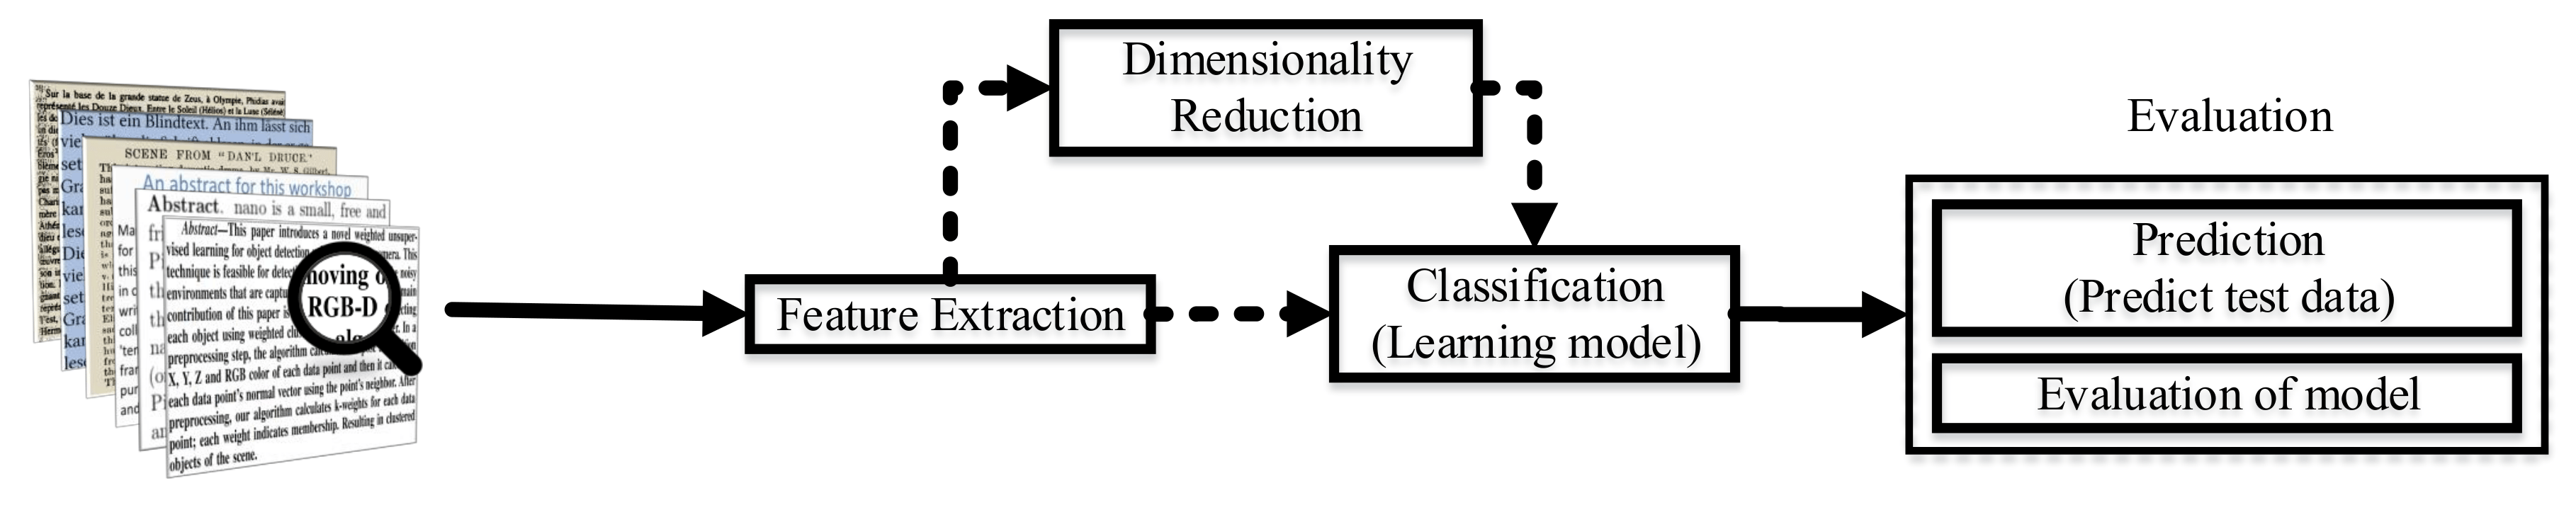
\includegraphics[width=1\textwidth]{img/pipeline.png}
    \caption{Overview of the text classification pipeline adopted from \cite{DBLP:journals/information/KowsariMHMBB19}.}
    \label{fig:pipeline}
\end{figure}
\fi

However, the advent of neural networks has shifted the focus away from the classical text classification pipeline just mentioned in favor of more novel deep learning approaches. This has resulted in manual feature extraction techniques such as Bag-of-Words and TF-IDF (Term Frequency-Inverse Document Frequency) becoming increasingly replaced with \textit{word embedding} methods \citep{DBLP:journals/csur/MinaeeKCNCG21}. Word embeddings are representations of words, typically in the form of real-valued, fixed-length vectors \citep{DBLP:journals/corr/abs-1901-09069}. In addition to methods such as Word2Vec \citep{DBLP:journals/corr/abs-1301-3781, DBLP:conf/nips/MikolovSCCD13} or GloVe \citep{DBLP:conf/emnlp/PenningtonSM14}, which are known as static word embeddings, there exist context-sensitive methods as of the late-2010s such as ELMo \citep{DBLP:conf/naacl/PetersNIGCLZ18} and BERT \citep{DBLP:conf/naacl/DevlinCLT19}, which can better represent the varied senses encompassed by words depending on their contexts.

Selecting an optimal model for the classification process itself also poses a crucial task. Without a comprehensive grasp of the underlying concepts of each algorithm, we cannot effectively determine an appropriate model for the task. Commonly known classical machine learning algorithms include Logistic Regression, Na\"ive Bayes and Support Vector Machines. More recently, deep learning models such as Convolutional Neural Networks (CNNs), Recurrent Neural Networks (RNNs) and Transformer Models have become established as state-of-the-art approaches, especially when considering large text classification tasks \citep{chen2015convolutional, DBLP:conf/ijcai/LiuQH16, DBLP:conf/aaai/LaiXLZ15, DBLP:conf/naacl/DevlinCLT19, DBLP:conf/cncl/SunQXH19}. One of the most well-established baseline transformer models is BERT \citep{DBLP:conf/naacl/DevlinCLT19}, which stands for Bidirectional Encoder Representations from Transformers. BERT was originally introduced with two different model sizes known as BERT\textsubscript{BASE} and BERT\textsubscript{LARGE}, both of which were pre-trained on the BooksCorpus dataset \citep{DBLP:conf/iccv/ZhuKZSUTF15} with 800 million words and English Wikipedia with 2,500 million words. Its bidirectional nature allows the model to learn a text's information from both the left and right context \citep{DBLP:conf/naacl/DevlinCLT19}. 

Generally, this pre-trained model can then be \textit{fine-tuned}, i.e., trained on additional data, for various more specific tasks. Looking to further improve upon this model, several variations of BERT have been presented since its creation, such as RoBERTa \citep{DBLP:journals/corr/abs-1907-11692} and SBERT \citep{DBLP:conf/emnlp/ReimersG19}. The latter, also known as Sentence-BERT, uses siamese and triplet network structures in order to produce sentence embeddings such that semantically similar sentences are close within the vector space, an aspect in which BERT was also shown to deliver unsuitable sentence embedding results for many common similarity measures \citep{DBLP:conf/emnlp/ReimersG19}. This approach has been further iterated upon by \cite{DBLP:setfit}, who proposed SetFit (Sentence Transformer Fine-tuning) as a framework for fine-tuning sentence transformers. The general idea of SetFit is to fine-tune a pre-trained SBERT model in a contrastive manner, then use this fine-tuned model to generate text embeddings for training \citep{DBLP:setfit}. 

The various deep learning methods just mentioned have become increasingly popular due to their ability to model more complex and nonlinear relationships within data \citep{DBLP:journals/nature/LeCunBH15}.
The Core-Set approach was also originally developed for the deep learning domain, particularly in the context of CNNs. As a result, this thesis focuses on the use of deep learning models, more specifically transformers.

Model evaluation is usually the ``final'' phase of the text classification process. This encompasses the assessment of the classifier's performance, for which a myriad of metrics such as accuracy, $\text{F}_1$-score and AUC can be employed. Based on the evaluation, one can select a suitable model/strategy as well as attempt to optimize it, e.g., by tuning hyperparameters.

The process of text classification clearly includes many steps which can be optimized and examined. For this reason, going over the entire process in detail would exceed the scope of this thesis. With this in mind, this thesis' experiment does not focus on the initial steps such as data collection, preprocessing, or generating embeddings, but rather the model training/fine-tuning and evaluation steps.

% **CHALLENGES(?)**

\section{Active Learning}

AL has become an increasingly important field when considering the need for efficient model construction as well as the labeling bottleneck in various machine learning tasks. Many fields, such as speech recognition, information extraction and classification suffer from this bottleneck as a result of their instance labels being expensive or time-consuming to obtain \citep{settles.tr09}. Generally, AL takes place in one of three main scenarios, namely \textit{membership query synthesis}, \textit{stream-based selective sampling} and \textit{pool-based active learning}. 

In the case of membership query synthesis, a membership query is created in the form of some unlabeled instance from the original dataset \citep{DBLP:journals/ml/Angluin87, DBLP:journals/ijon/WangHYL15}. In other words, this approach synthesizes a query \textit{de novo}, rather than selecting some query from the instance space \citep{settles.tr09}. One challenge of this approach is ensuring that the synthesized query is consistent with meeting the constraints imposed by the real data. In the case of a human oracle, this can result in unrecognizable queries, for example in the case of computer vision tasks \citep{langbaum92}. Similarly, this issue could also apply to text classification, where query synthesis might produce unintelligible texts \citep{settles.tr09}.

Stream-based selective sampling, in contrast, typically examines each unlabeled instance one at a time and decides whether to query the oracle or to assign a label \citep{settles.tr09}. This concept has been applied to various tasks such as sensor scheduling \citep{DBLP:journals/tsp/Krishnamurthy02} or sentiment analysis for stock price predictions \citep{DBLP:journals/isci/SmailovicGLZ14}.

\begin{figure}[htbp]
    \centering
    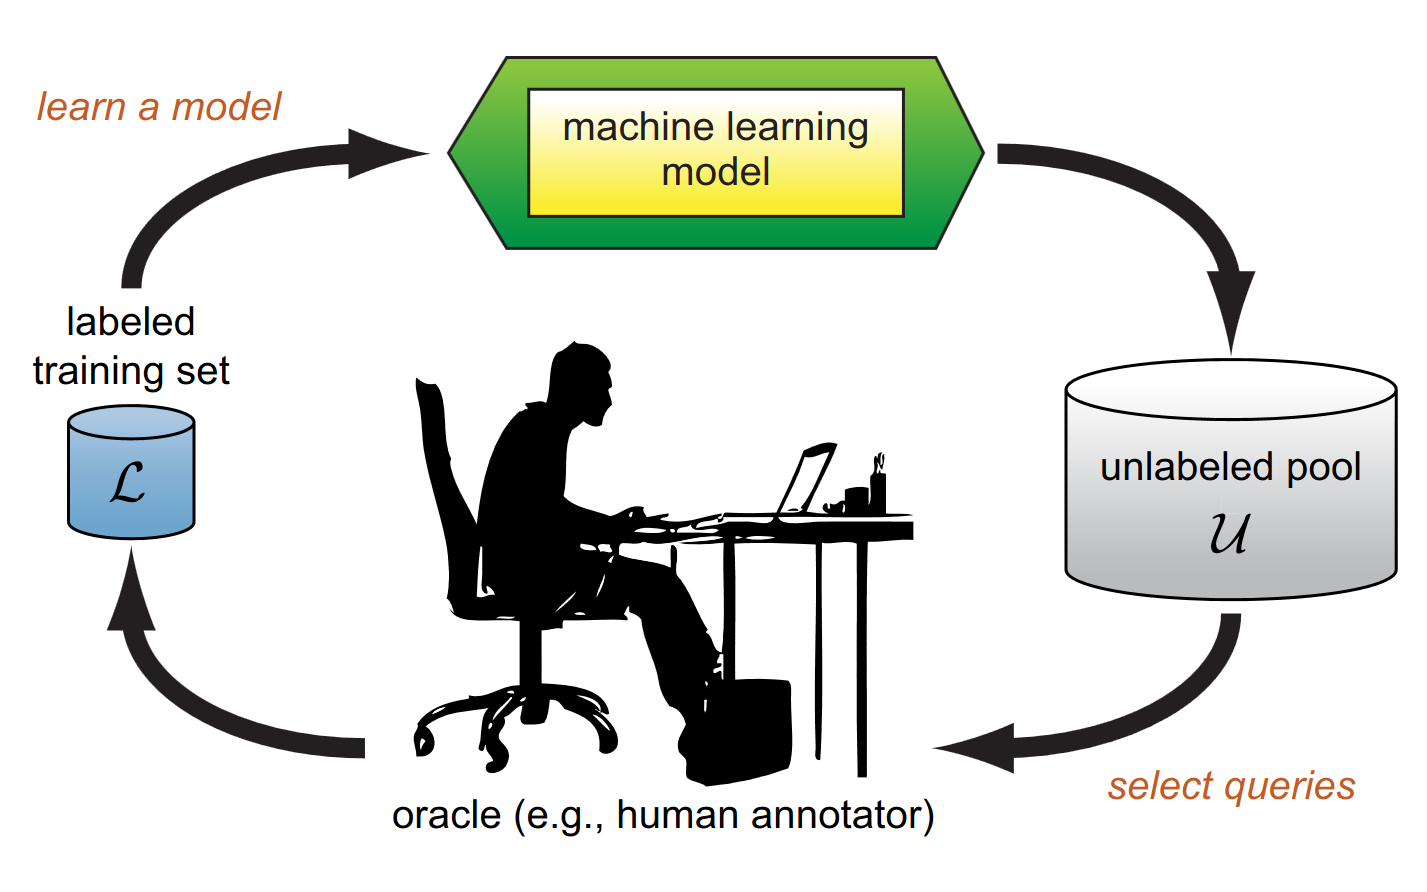
\includegraphics[width=0.7\textwidth]{img/al.png}
    \caption{Overview of the pool-based AL scenario adopted from \cite{settles.tr09}.}
    \label{fig:activelearning}
\end{figure}

Finally, we consider the pool-based approach (illustrated in Figure~\ref{fig:activelearning}) as one of the commonly known applications of AL. This scenario assumes a large set of unlabeled instances and a small set of labeled instances, from which queries can be selectively drawn using a query strategy. Generally, most approaches begin with some random selection of points to initialize the classifier. With each AL iteration, the query strategy selects new instances on which to train the classifier. This process is then repeated until some stopping criterion is met. 

The key difference to the stream-based approach is that pool-based learning considers the entire collection and attempts to select the most informative instances, as opposed to making individual query decisions. This can be useful in many real-world problems where plenty of unlabeled data is available and the pool is assumed to be closed (though this is not necessarily always the case) \citep{settles.tr09}.

This thesis considers the case of the pool-based scenario, as does the original Core-Set paper. It is worth mentioning, however, that Core-Set has also been applied in the stream-based context \citep{DBLP:conf/icml/SaranYK0A23}.

\section{Core-Set}

The Core-Set approach as proposed by \cite{DBLP:conf/iclr/SenerS18} was originally designed for CNNs to tackle the task of performing AL on large datasets. The empirical studies conducted in this paper show that Core-Set outperforms other established query strategies when applied in the field of computer vision.

\cite{DBLP:conf/iclr/SenerS18} define the task of AL as a \textit{core-set selection} problem in which the algorithm selects a smaller subset of points with increased diversity to learn from such that the model can be competitive over a larger dataset. This problem ends up being equivalent to the \textit{k-Center problem}, which is also referred to as the minimax facility location problem \citep{DBLP:conf/iclr/SenerS18}. 

In mathematical terms, given a set of points $ [n] $ and a budget $ k \leq |[n]| $, $k$-Center finds a subset $ \mathbf{s} \subseteq [n] $ of $ k $ points such that the maximum distance of any point in $ [n] \setminus \mathbf{s} $ to its closest center in $ \mathbf{s} $ is minimal \citep{har2008geometric}.\footnote{Following the notation of \cite{DBLP:conf/iclr/SenerS18}, $ [n] $ denotes the indices referring to the collection of data points.} Core-Set applies this concept to the field of AL in that the $ k $ centers selected from $ [n] $ will be the instances selected for labeling by the oracle (the amount of selected centers is also referred to by \cite{DBLP:conf/iclr/SenerS18} as the \textit{budget}, or $ b $). Note that \cite{DBLP:conf/iclr/SenerS18} employs the $ l_2 $ norm (Euclidean distance) for the distance metric $ \Delta(\cdot, \cdot) $. 

\vspace{0.2\baselineskip}

\begin{figure}[htbp]
    \centering
    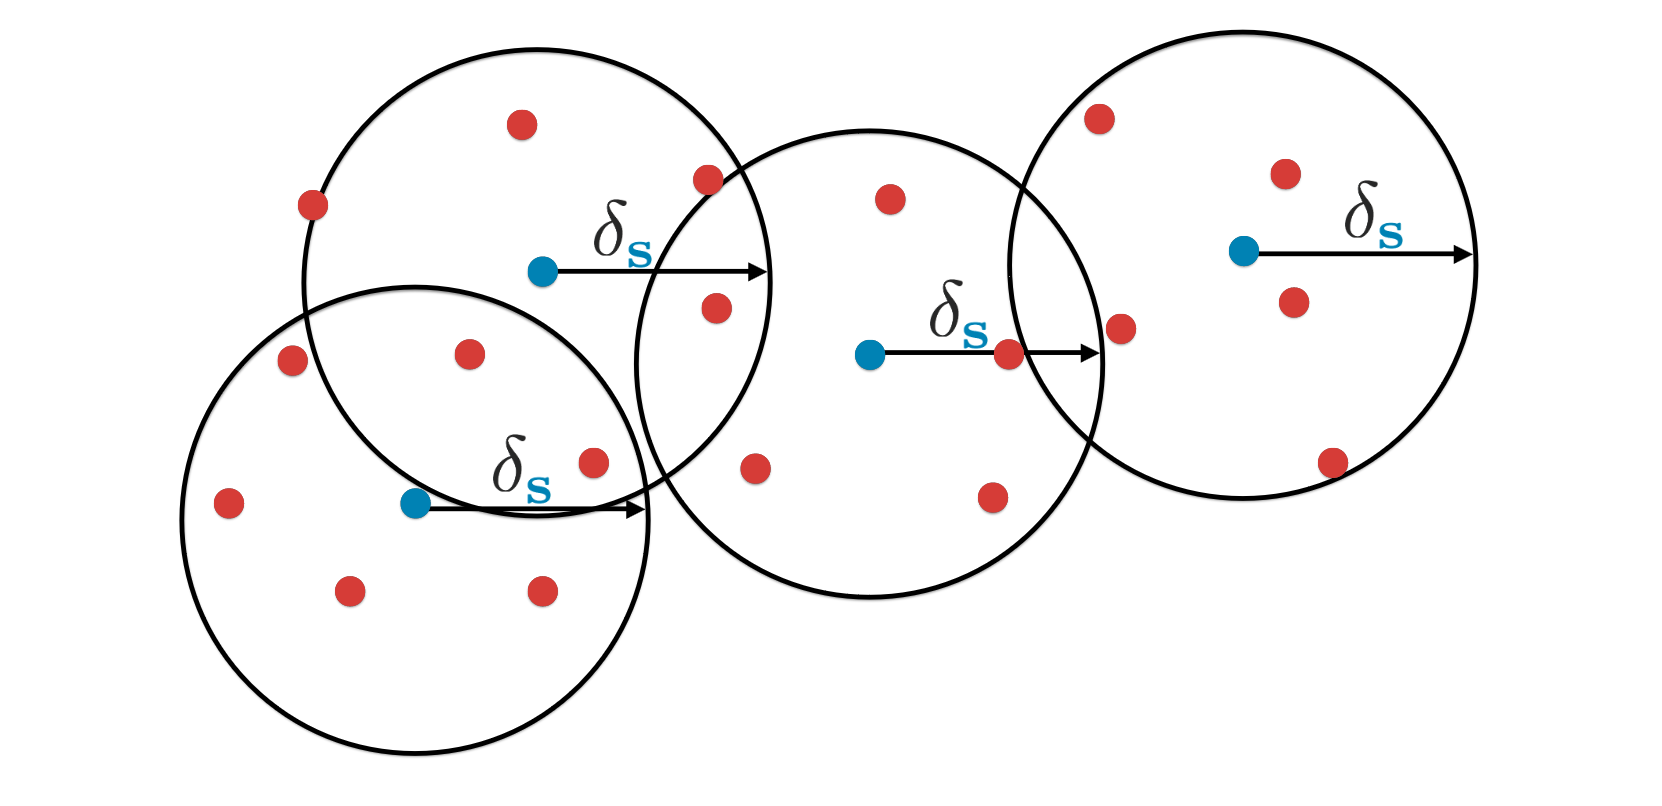
\includegraphics[width=1\textwidth]{img/coreset.png}
    \caption{Visualization of the $k$-Center approach from \cite{DBLP:conf/iclr/SenerS18}. $ \mathbf{s} $ denotes the set of $ k $ selected points, $ \delta_{\mathbf{s}} $ denotes the maximum distance of any point in $ [n] \setminus \mathbf{s} $ to its nearest center in $ \mathbf{s} $.}
    \label{fig:coreset}
\end{figure}

Another way of viewing this problem is by placing circles around the points in our set of centers. If we denote the maximum distance of any point in $ [n] \setminus \mathbf{s} $ to its nearest center in $ \mathbf{s} $ with $ \delta_{\mathbf{s}} $, and we place circles with a $ \delta_{\mathbf{s}} $-radius around each center in $ \mathbf{s} $, we can ``cover'' the entire set of points $ [n] $. In other words, $k$-Center attempts to find the minimum $ \delta_{\mathbf{s}} $ such that all points lie within the union of the $ \delta_{\mathbf{s}} $-circles when placed upon each center (depicted in Figure~\ref{fig:coreset}). Due to the nature of $k$-Center, the selected points tend to be spread out throughout the dataset in order to ``cover'' all the unselected points, making this a diversity-based approach. 

This problem has been shown to be NP-hard \citep{DBLP:journals/dam/HsuN79, DBLP:journals/anor/Hochbaum84}. The Core-Set approach opts for a greedy approach to solve the $k$-Center problem. However, it is worth noting that any approximation of $k$-Center is bound by twice the optimal solution \citep{DBLP:journals/dam/HsuN79}. Let $ OPT $ denote the maximum distance of a center to a point in the optimal solution to $k$-Center, meaning the solution where $\delta_{\mathbf{s}} $ is minimal. Then the greedy approximation's resulting maximum distance $ \delta_{\mathbf{s}} $ to any center in $ \mathbf{s} $ is at the worst $ 2 \cdot OPT $ \citep{mountkcenter}. The pseudocode used by \cite{DBLP:conf/iclr/SenerS18} for $k$-Center greedy within the AL context can be seen in Algorithm~\ref{alg:coreset}.

\vspace{0.4\baselineskip}

\begin{algorithm}[htpb]
    \caption{$k$-Center-Greedy (adopted from \cite{DBLP:conf/iclr/SenerS18})}%
%\makeatletter\def\@currentlabel{CS}\makeatother
\label{alg:coreset}

\begin{algorithmic}

\Require data $ \mathbf{x}_i $, existing pool $ \mathbf{s}^0 $, budget $ b $
\State Initialize $ \mathbf{s} = \mathbf{s}^0 $
\Repeat
\State $ u = \text{argmax}_{i \in [n] \setminus \mathbf{s}} \text{min}_{j \in \mathbf{s}} \Delta(\mathbf{x}_i, \mathbf{x}_j) $
\State $ \mathbf{s} = \mathbf{s} \cup \{u\} $
\Until{$ |\mathbf{s}| = b + |\mathbf{s}^0|$}

\State \textbf{return} $\mathbf{s} \setminus \mathbf{s}^0 $
\end{algorithmic}
\end{algorithm}

\vspace{0.3\baselineskip}

The original paper by \cite{DBLP:conf/iclr/SenerS18} attempts to further improve the robustness of this approximation by placing an upper limit on the number of outliers that can be selected. This thesis focuses on and uses the regular $k$-Center greedy algorithm, which is generally better established due to ease of implementation and interpretability.

\section{Dimensionality Reduction}

As pointed out earlier, one of the challenges of the Core-Set approach is handling data points with a higher dimensionality \citep{DBLP:conf/iccv/SinhaED19}. Broadly speaking, this is a phenomenon coined by Richard E. Bellman known as the \textit{curse of dimensionality} \citep{Freimer1961AdaptiveCP}, which has been observed to negatively impact the contrast of proximities for distance-based problems such as nearest-neighbors \citep{DBLP:conf/icdt/BeyerGRS99, DBLP:books/lib/HastieTF09}. In relation to this, \cite{DBLP:conf/icdt/AggarwalHK01} point out that the $ l_2 $ norm is not preferable in higher dimensions and \cite{DBLP:conf/iwann/VerleysenF05} conclude that standard Euclidean norms may become unselective in these cases.

As a result, many algorithms have been developed to transform data from a high-dimensional space into a low-dimensional space. Moreover, reducing dimensionality is often an important aspect when considering the task of data visualization. This task directly poses another challenge: managing to reduce the dimensionality of the data while still being able to retain the highest possible amount of information. 

One such method is the Principal Components Analysis (PCA), which is one of the most popular linear techniques for dimensionality reduction \citep{van2009dimensionality}. In essence, PCA linearly transforms the data into a representation that attempts to closely describe the variance of the initial data \citep{jolliffe2016principal}. Other commonly used linear techniques include Linear Discriminant Analysis (LDA), Multidimensional Scaling (MDS), and Non-negative Matrix Factorization (NMF).

These techniques can be powerful; however, they often miss important nonlinear structures in high-dimensional data \citep{Tenenbaum2000AGG}. This motivates the development of nonlinear techniques such as Isometric Mapping (Isomap), t-distributed Stochastic Neighbor Embedding (t-SNE) and Uniform Manifold Approximation and Projection (UMAP). 

\subsection*{t-distributed Stochastic Neighbor Embedding}

t-SNE is a relatively modern probabilistic approach that has improved upon many other nonlinear techniques in creating a single map that reveals structure on many different scales. In addition, it manages to reduce the tendency of Stochastic Neighbor Embedding (SNE) to crowd data points together at the center by using a different cost function \citep{van2008visualizing}. 

First, it converts the high-dimensional Euclidean distances into conditional probabilities, such that similar data points are assigned higher probabilities and dissimilar data points are assigned very low probabilities. It then creates a similar probability distribution over the lower-dimensional map such that the \textit{Kullback--Leibler divergence} (a measure of how one probability distribution differs from another) is minimized. 

The caveat of this technique is that its efficiency on large datasets relies on a variant of the Barnes--Hut algorithm, which results in reductions only being possible to the two- or three-dimensional space \citep{DBLP:journals/corr/abs-1301-3342}. Because of this drawback, the method is often used for the visualization of high-dimensional data, for which a reduction to two- or three- dimensional spaces is ideal.

\subsection*{Uniform Manifold Approximation and Projection}

UMAP exists in a similar vein to t-SNE, but offers important improvements in some areas. It models the data with a fuzzy topological representation using simplices, then attempts to find some low-dimensional projection with the closest possible equivalent fuzzy topological structure \citep{DBLP:journals/corr/abs-1802-03426}. Another key difference is that UMAP accomplishes this projection by attempting to minimize the cross-entropy between the topological representations, whereas t-SNE uses the Kullback--Leibler divergence. 

\cite{DBLP:journals/corr/abs-1802-03426} also elaborate that the resulting reductions are competitive with t-SNE in the field of visualization and offer superior runtime performances. In addition, there exists no computational restriction on the embedding dimension, as opposed to t-SNE. As a result, \cite{DBLP:journals/corr/abs-1802-03426} mention it as a useful tool not only for visualization, but for machine learning tasks in general.

\chapter{Approach}

The following chapter describes my approach to the subsequent experiment. The attempt to improve upon and modify Core-Set resulted in multiple different iterations of the original $k$-Center greedy algorithm, which I have grouped into three different categories. Each of these different categories is designed to address one of the three research questions central to this thesis. 

First, I outline the dimensionality reduction-based approach, considering the two different nonlinear techniques (t-SNE and UMAP) discussed previously. After that, I present two uncertainty-based approaches that take pointwise probabilities into account. The final approach for the experiment attempts to use class balancing in combination with Core-Set.

\section{Dimensionality Reduction-Based}

As mentioned in Section 2.4, distinctions in distance decrease with higher dimensions \citep{DBLP:conf/icdt/BeyerGRS99}, and more specifically, previous work has observed Core-Set to become less effective in higher dimensions \citep{DBLP:conf/iccv/SinhaED19}.

As a solution to this, I propose the application of a nonlinear dimensionality reduction technique on the training data before selecting new points using Core-Set. My aim with this is to attempt to overcome the curse of dimensionality, and in the process of doing this, preserve any nonlinear structures within the datasets. This modification to the original $k$-Center greedy algorithm is relatively straightforward and is denoted by $ \Delta_{Reduced} $ in Algorithm~\ref{alg:coreset-dr}, signifying the distances between the reduced embeddings.

\begin{algorithm}[htpb]
\caption{Dimensionality-Reduced $k$-Center-Greedy}%
%\makeatletter\def\@currentlabel{CS-tSNE}\makeatother
\label{alg:coreset-dr}
\begin{algorithmic}


\Require data $ \mathbf{x}_i $, existing pool $ \mathbf{s}^0 $, budget $ b $
\State Initialize $ \mathbf{s} = \mathbf{s}^0 $
\Repeat
\State $ u = \text{argmax}_{i \in [n] \setminus \mathbf{s}} \text{min}_{j \in \mathbf{s}} \Delta_{Reduced}(\mathbf{x}_i, \mathbf{x}_j) $
\Comment{Computing distances on}
\State $ \mathbf{s} = \mathbf{s} \cup \{u\} $
\Comment{reduced embeddings}
\Until{$ |\mathbf{s}| = b + |\mathbf{s}^0|$}

\State \textbf{return} $\mathbf{s} \setminus \mathbf{s}^0 $
\end{algorithmic}
\end{algorithm}

This resulted in two dimensionality-reduction based approaches. The first strategy, which I refer to as CS--tSNE, uses t-SNE in order to reduce the embeddings down to two dimensions. Additionally, I propose the use of UMAP as an alternative technique, which I employ to reduce the data to a 256-dimensional space.\footnote{Both of these approaches will operate on 768-dimensional embeddings.} This strategy will be referred to as CS--UMAP. The choice of these two reduction dimensions aims to examine the possible differences in performance for a reduction to a low-dimensional space in the case of t-SNE and a comparatively high-dimensional reduction in the case of UMAP. The reason for using these two different techniques is a result of t-SNE's limitations concerning the dimension of the reduced space explained briefly in Section 2.4.

\section{Uncertainty-Based}

\cite{DBLP:conf/iclr/SenerS18} state that their approach does not consider any uncertainty information. With this in mind, I propose an approach to examine the effect of pointwise probabilities on the Core-Set algorithm. Core-Set currently operates using the distances between its points -- in this experiment, I aim to modify Core-Set such that it considers the probability distributions in addition to the distances.

To accomplish this, I use an uncertainty-based approach. Uncertainty sampling, which was introduced by \cite{DBLP:conf/sigir/LewisG94}, essentially attempts to select the unlabeled examples with the lowest classification certainty. In this case, I specifically opted for an approach similar to that of Breaking-Ties \citep{DBLP:journals/jmlr/LuoKGHSRH05}, where the instances with the smallest margin between their top two most likely classification probabilities are selected, essentially ``breaking the tie'' between the two most likely classes. In other words, if $ \mathbf{p}_{j, k}^* $ denotes the probability of the $ k $-th most likely class label for the $ j $-th instance, then Breaking-Ties seeks to select instances where $ \mathbf{p}_{j, 1}^* - \mathbf{p}_{j, 2}^* $ is minimal.

\begin{algorithm}[htpb]
\caption{Weighted $k$-Center-Greedy}%
%\makeatletter\def\@currentlabel{WCS}\makeatother
\label{alg:wgc}
\begin{algorithmic}

\Require $ \mathbf{x}_i $, $ \mathbf{s}^0 $, $ b $, Breaking-Ties probabilities $ \mathbf{p}_{bt} $
\State Initialize $ \mathbf{s} = \mathbf{s}^0 $
\Repeat
\State $ d = \text{min}_{j \in \mathbf{s}} \Delta(\mathbf{x}_i, \mathbf{x}_j) $ 
    \State $ u = \text{argmax}_{i \in [n] \setminus \mathbf{s}} 0.8 \cdot d + 0.2 \cdot \mathbf{p}_{bt} $
    \Comment{Weigh results using linear}
\State $ \mathbf{s} = \mathbf{s} \cup \{u\} $
\Comment{combination}
\Until{$ |\mathbf{s}| = b + |\mathbf{s}^0|$}

\State \textbf{return} $\mathbf{s} \setminus \mathbf{s}^0 $
\end{algorithmic}
\end{algorithm}

This approach resulted in two different implementation ideas: the first, which I will refer to as ``Weighted Core-Set'' (WCS, depicted in Algorithm~\ref{alg:wgc}), computes the uncertainties prior to querying, then multiplies the resulting Core-Set distances and probabilities using weights during selection (in this case, I used an 80--20 weighting in favor of the Core-Set distances).

The second, which I will call ``Re-ranked Core-Set'' (RCS, depicted in Algorithm~\ref{alg:rwgc}), opts to first compute a Core-Set twice the size of the original sample size $b$, then ``re-ranks'' the resulting distances according to Breaking-Ties uncertainties and finally selects the points with the $b$ highest uncertainties.

In theory, these two approaches aim to use uncertainties to improve Core-Set's selections, such that the newly selected set of points should ideally contain instances which also have high uncertainties. A similar concept, dubbed ``hybrid query strategy'' has been investigated by \cite{DBLP:journals/corr/abs-2110-03785} previously. In this case, the ``combination'' of multiple approaches hopes to utilize the benefits of each one within a single strategy.

\begin{algorithm}[htpb]
\caption{Re-ranked $k$-Center-Greedy}%
%\makeatletter\def\@currentlabel{RCS}\makeatother
\label{alg:rwgc}
\begin{algorithmic}

\Require $ \mathbf{x}_i $, $ \mathbf{s}^0 $, $ b $, class probabilities $ \mathbf{p}_i $
\State Initialize $ \mathbf{s} = \mathbf{s}^0, r = \emptyset $
\Repeat
\State $ u = \text{argmax}_{i \in [n] \setminus \mathbf{s}} \text{min}_{j \in \mathbf{s}} \Delta(\mathbf{x}_i, \mathbf{x}_j) $
\State $ \mathbf{s} = \mathbf{s} \cup \{u\} $
\Until{$ |\mathbf{s}| = 2b + |\mathbf{s}^0|$}
\Comment{Compute Core-Set of size $2b$}

%\State $ \mathbf{p}_{bt} = \text{breaking\_ties}_{i \in \mathbf{s}}(\mathbf{p}_i) $

%\State $ \mathbf{s} = \mathbf{s} \cap \text{argpartition}(\mathbf{p}_{bt}, b) $

\Repeat
\State $ u = \text{argmin}_{j \in \mathbf{s} \setminus r}\mathbf{p}_{j, 1}^* - \mathbf{p}_{j, 2}^* $
\State $ r = r \cup \{u\} $
\Until{$ |r| = b $}
\Comment{Compute the $b$-highest BT-scores}

\State \textbf{return} $ r $
\end{algorithmic}
\end{algorithm}

\section{Class Balance-Based}

Finally, I take into account the class distributions within each Core-Set and select points based on the representation of each class. This approach will be called ``Class-Balanced Core-Set'' (CB--CS).

\begin{algorithm}[htpb]
    \caption{Class-Balanced $k$-Center Greedy}%
%\makeatletter\def\@currentlabel{CB-CS}\makeatother
\label{alg:classbalanced}
\begin{algorithmic}

\Require $ \mathbf{x}_i $, $ \mathbf{s}^0 $, $ b $, true class labels $ y_i $, predicted class labels $ y^{pred}_i $, classes $ C $

\State $ d = \text{target\textunderscore dist}_{i \in [n] \setminus \mathbf{s}} (b, C, y_i, y^{pred}_i) $

\State Initialize $ \mathbf{s} = \mathbf{s}^0 $
\For{$c \in C$}
\State $ \mathbf{s}^c = \emptyset $
% \State $ \text{class\textunderscore indices} = \{i \; | \; y_i^{pred} = c\} $
\State $ \text{class\textunderscore pool} = \{i \in [n] \setminus \mathbf{s} \; | \; y_i^{pred} = c\} $
\Repeat
\State $ u = \text{argmax}_{i \in \text{class\textunderscore pool}}\text{min}_{j \in \mathbf{s}} \Delta(\mathbf{x}_i, \mathbf{x}_j) $
\State $ \mathbf{s}^c = \mathbf{s}^c \cup \{u\} $
\Until{$ |\mathbf{s}^c| = d^c $}
\Comment{Select desired amount}
\State $ \mathbf{s} = \mathbf{s} \cup \mathbf{s}^c $
\Comment{of instances for class $c$}
\EndFor

\State \textbf{return} $ \mathbf{s} \setminus \mathbf{s}^0 $
\end{algorithmic}
\end{algorithm}

Imbalanced class distributions within training data can pose a problem for text classification \citep{DBLP:conf/eacl/HenningBFF23}. Accordingly, the basic idea behind this approach is to select unlabeled instances so that the class distribution within the pool of labeled instances is even. In other words, this iteration of Core-Set will attempt to select more or less instances of a certain class depending on the discrepancy between the current class distribution of the labeled pool and the desired uniform distribution.

One way of determining the degree to which our pool of instances is ``class-balanced'' is by using the normalized entropy metric with respect to the normalized histogram of the labeled pool's classes. This metric is based on the Shannon entropy $ H $ \citep{DBLP:journals/bstj/Shannon48}, which is defined in Equation~\ref{eq:entropy} over some discrete random variable $ X $, which is in this case the class distribution.

\begin{equation}\label{eq:entropy}
    H(X) = -\sum_{x \in X} p(x) \log p(x)
\end{equation}

\noindent Dividing by the logarithm of the number of classes $n$ for the class distribution, we get the normalized entropy $ H_{norm} $(Equation~\ref{eq:nentropy}), also referred to as $ H_{REL} $ by \cite{wilcox1967indices}.

\begin{equation}\label{eq:nentropy}
    H_{norm}(X) = \frac{-\sum_{x \in X} p(x) \log p(x)}{\log n}
\end{equation}

\noindent This metric scales the output to lie between 0 and 1, such that 1 indicates a uniform distribution. This can be applied to the measurement of class imbalances, where a normalized entropy value closer to 1 indicates a more balanced class distribution and is therefore a desirable result. Thus, the aim of this approach is to increase this metric with each iteration such that the classes are balanced within the labeled pool.\footnote{Note that the instance selection takes place with respect to the \textit{predicted} class labels $ y^{pred} $, so perfect selections cannot be guaranteed.}

To this end, I divide a single query into multiple Core-Set computations, essentially constructing disjoint Core-Set selections for each class. For each class' Core-Set selection, the budget $ b $ (e.g., the number of selected instances from this class) depends on the desired class distribution. First, the class distributions of the model's predictions and of the true labels are used to determine how many instances should ideally be queried for each class in order to achieve a ``class balance'' in the labeled pool. In the corresponding pseudocode (Algorithm~\ref{alg:classbalanced}), this calculation has been denoted by the use of \texttt{target\textunderscore dist}, which uses an existing implementation from the Python library small-text \citep{schroeder2023small-text}. The resulting distribution $ d $ then contains the desired number of instances for each class $ c \in C $, denoted by $ d^c $. After this, $k$-Center greedy is used to select the desired number of points of each class, such that if $ d^c $ denotes the number of newly selected instances for the class $ c $, then $ \sum_{c \in C} d^c = b $. 

\chapter{Experiment}

With these approaches in mind, this chapter outlines the experiment, first describing the data and setup of the experiment and finally delving into its results. 

This experiment takes place within a simulated AL environment, meaning the oracle is not a human expert or annotator but rather an already labeled pool of data. To this end, I select three established pre-labeled text classification datasets differing in text genre and class cardinalities. The AL takes place on these datasets using two different classification models, each of which I then combine with one of eight different query strategies: two baselines, the Core-Set approach, and five previously introduced Core-Set variants.

The following two sections explain in greater detail the data and setup used as a basis for the conducted experiment. The performances are then measured using two metrics, accuracy and AUC, throughout five runs for each combination of dataset, model, and query strategy. The accuracy metric describes the number of correct predictions made by the model divided by the total number of predictions and can thus give an indication of how well the model predicts an instance's label. AUC, or ``Area Under Curve'', describes the area under the learning curve, which may give some measure of how quickly the model's performance improves during the learning process. In the final section, I present and evaluate the experiment results.

\section{Data}

This experiment was conducted across three datasets commonly used in the field of text classification. These datasets are of three different types: sentiment analysis, questions, and news. 

For binary classification, I used \textbf{Movie Review} \citep{DBLP:conf/acl/PangL05}, a sentiment analysis dataset containing 5,331 positive and 5,331 negative online movie reviews. For multi-class text classification, I performed the AL on \textbf{AG's News} \citep{DBLP:conf/nips/ZhangZL15}, a news dataset comprised of 120,000 training samples and 7,600 test samples, and \textbf{TREC} \citep{DBLP:journals/nle/LiR06}, a question dataset containing 5,500 training samples and 500 test samples. The test set was provided in the case of AG's News and TREC; in the case of Movie Review I employed a split of the 10,662 samples myself, which can be seen alongside additional information in Table~\ref{tab:dataset-table}. Example instances from each dataset as well as their corresponding classes can also be seen in Table~\ref{tab:dataset-instances}.

\vspace{1\baselineskip}

\begin{table}[htpb]
    \centering
    \setlength{\tabcolsep}{16pt} % Adjust the spacing between columns
    \begin{tabular}{@{}lrrrr@{}} % use @{} to remove spacing; numbers should be right aligned
        \toprule
        % \multicolumn{4}{c}{\bfseries Some numbers}\\
        % \midrule
        \bfseries Dataset Name \scriptsize (ID) & \bfseries Classes & \bfseries Train & \bfseries Test & \bfseries MNC (*) \\
        % \cmidrule(l){2-4} % cmidrule: A line from 2nd to 4th column, trimmed on the left hand side
        \midrule
        Movie Review \scriptsize (MR) & 2 & 9,596 & 1,066 & 114.16 \\
        AG News \scriptsize (AGN) & 4 & 120,000 & 7,600 &  236.41 \\
        TREC \scriptsize (TREC) & 6 & 5,500 & 500 & 49.39 \\
        \bottomrule
    \end{tabular}
    \caption{Information on the different datasets. (*) Mean number of characters in a single instance.}
  \label{tab:dataset-table}%
\end{table}

\vspace{1\baselineskip}

\begin{table}[htbp]
    \centering
    \renewcommand{\arraystretch}{1.5}
    \begin{tabular}{@{}lrp{7cm}@{}} 
        \toprule
        \textbf{Dataset Name} \scriptsize (ID) & \textbf{Class} & \textbf{Example Instance} \\
        \midrule
        Movie Review \scriptsize (MR) & 1 (positive) & \texttt{if you sometimes like to go to the movies to have fun , wasabi is a good place to start .} \\
        AG News \scriptsize (AGN) & 2  (Business) & \texttt{Wall St. Bears Claw Back Into the Black (Reuters) Reuters - Short-sellers, Wall Street's dwindling\textbackslash band of ultra-cynics, are seeing green again.} \\
        TREC \scriptsize (TREC) & 2 ('DESC') & \texttt{How did serfdom develop in and then leave Russia ?} \\
        \bottomrule
    \end{tabular}
    \caption{Examples of instances and their corresponding labels from each dataset. The label 'DESC' signifies a description or abstract concept.}
    \label{tab:dataset-instances}
\end{table}

\newpage 

\section{Experiment Setup}

I selected two state-of-the-art transformer models, BERT \citep{DBLP:conf/naacl/DevlinCLT19} and SetFit \citep{DBLP:setfit} to fine-tune for this experiment. BERT is an established language model pre-trained on 3,300 million English words and may thus serve as a good baseline model for this experiment. It uses bidirectional self-attention in order to incorporate context from both directions of a given token, unlike many previous context-sensitive approaches, which only considered a single direction. For this experiment, I use BERT\textsubscript{BASE}, which consists of 12 layers, hidden units of size 768 with 110 million parameters in total. By contrast, SetFit is based on sentence transformers, which are then fine-tuned in a contrastive manner. This model also has 12 layers and 110 million parameters, and it generates 768-dimensional embeddings. Due to the nature of sentence transformers explained previously in Section 2.1, this model may be able to aid Core-Set's selection as a consequence of the improved vector space representations when considering similarity measures \citep{DBLP:conf/emnlp/ReimersG19}. The model implementations used in this experiment are HuggingFace's \href{https://huggingface.co/google-bert/bert-base-uncased}{bert-base-uncased} and \href{https://huggingface.co/sentence-transformers/paraphrase-mpnet-base-v2}{
paraphrase-mpnet-base-v2}.

The experiment is conducted by performing 20 queries with 25 instances, starting with an initialized pool of size 25. The results are averaged over five runs of queries per combination of dataset, model, and query strategy. The training and evaluation of these models is run using an AL experiment setup based on the Python library small-text \citep{schroeder2023small-text}. This library also includes the implementation of $k$-Center greedy as well as various methods concerning class redistributions.

Alongside the original Core-Set (CS), I compare my different approaches with Random Sampling (RS) and Breaking-Ties (BT).\footnote{In the following, ``CS'' refers to the query strategy itself within the context of the experiment, whereas ``Core-Set'' refers to the approach as a concept.} RS offers a good view of a baseline performance and is especially of interest when compared to Core-Set. BT, on the other hand, may serve as a good reference when looking at improving Core-Set's performance.

\section{Experiment Results}

% Based on the experimental setup outlined in Section 4.2, this chapter presents the outcomes for each experiment run. Section 4.3.1 will show the learning curves for the each training run, and Section 4.3.2 will report on the corresponding result tables.
Based on the experimental setup outlined in Section 4.2, this chapter presents the outcomes for each experiment run. I first present the learning curves for each training case, then compare the strategies regarding their final accuracy and AUC scores.

\iffalse
%% TEMPLATE TABLE
\begin{table*}[h!]%
\centering
\fontsize{8pt}{9pt}\selectfont%
\renewcommand{\tabcolsep}{12pt}%
\begin{tabular}{@{}ll@{\hspace{10pt}} r @{${}\pm{}$} r r @{${}\pm{}$} r r @{${}\pm{}$} r r @{${}\pm{}$} r @{}}
\toprule
\textbf{Dataset} & \textbf{Model} & \multicolumn{8}{c}{\textbf{Query Strategy}}\\
\cmidrule{3-10} & & \multicolumn{2}{c}{\hspace*{-6pt}RS} & \multicolumn{2}{c}{BT} & \multicolumn{2}{c}{CS} & \multicolumn{2}{c}{\hspace*{4pt}Unknown}\\
\midrule
\multirow{2}{*}{AGN}  & BERT & 1.852 & 0.415 & 0.907 & 0.203 & \bfseries 0.432 & \bfseries 0.097 & 516.554 & 115.583 \\
 & SetFit & 7.264 & 1.626 & \bfseries 6.199 & \bfseries 1.389 & 10.256 & 2.359 & 481.758 & 142.013 \\
\midrule
\multirow{2}{*}{MR}  & BERT & 0.014 & 0.003 & 0.014 & 0.003 & \bfseries 0.009 & \bfseries 0.002 & 1.889 & 0.425\\
 & SetFit & 0.521 & 0.117 & \bfseries 0.436 & \bfseries 0.098 & 0.468 & 0.105 & 3.672 & 1.098 \\
\midrule
\multirow{2}{*}{TREC-6}  & BERT & 0.085 & 0.019 & 0.042 & 0.009 & \bfseries 0.018 & \bfseries 0.004 & 0.609 & 0.138 \\
 & SetFit & 0.289 & 0.065 & \bfseries 0.248 & \bfseries 0.055 & 1.111 & 0.745 & 1.504 & 0.447 \\
\bottomrule
\end{tabular}
\caption{%
Final accuracy per dataset, model, and query strategy. We report the mean and standard deviation over five runs. The best result per dataset is printed in bold.}
\label{table-results-acc}
\end{table*}
\fi

\subsection*{Learning Curves}

%The following figures show the learning curves for each combination of dataset, model and query strategy. 

% CROPPED IMAGES
\begin{figure}[t]
    \centering
    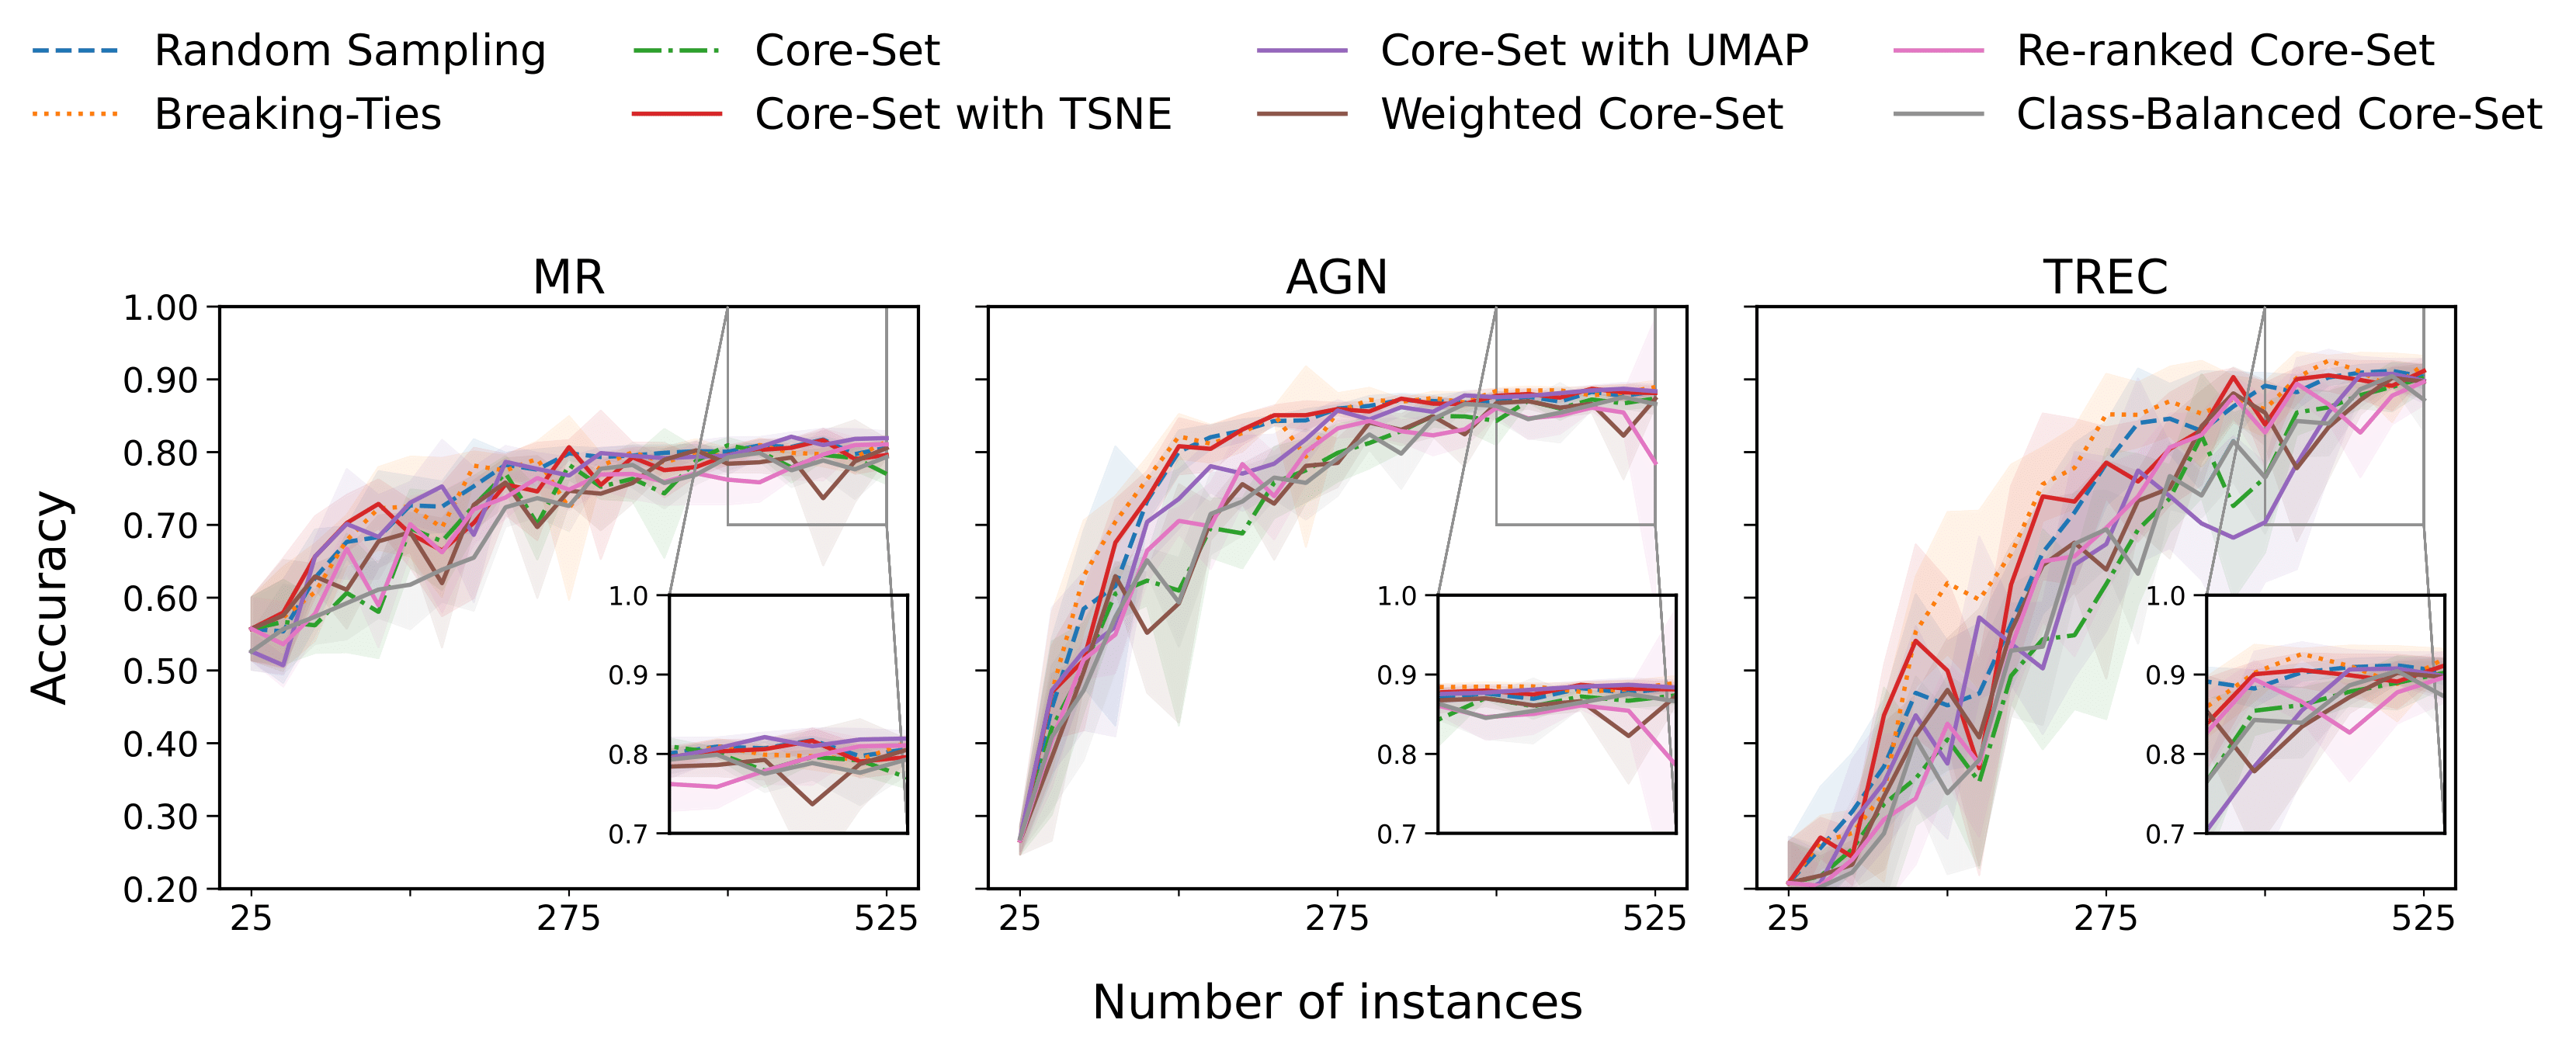
\includegraphics[width=1\textwidth,trim={0 1.1cm 0 0},clip]{img/bert-plots-1.png}
    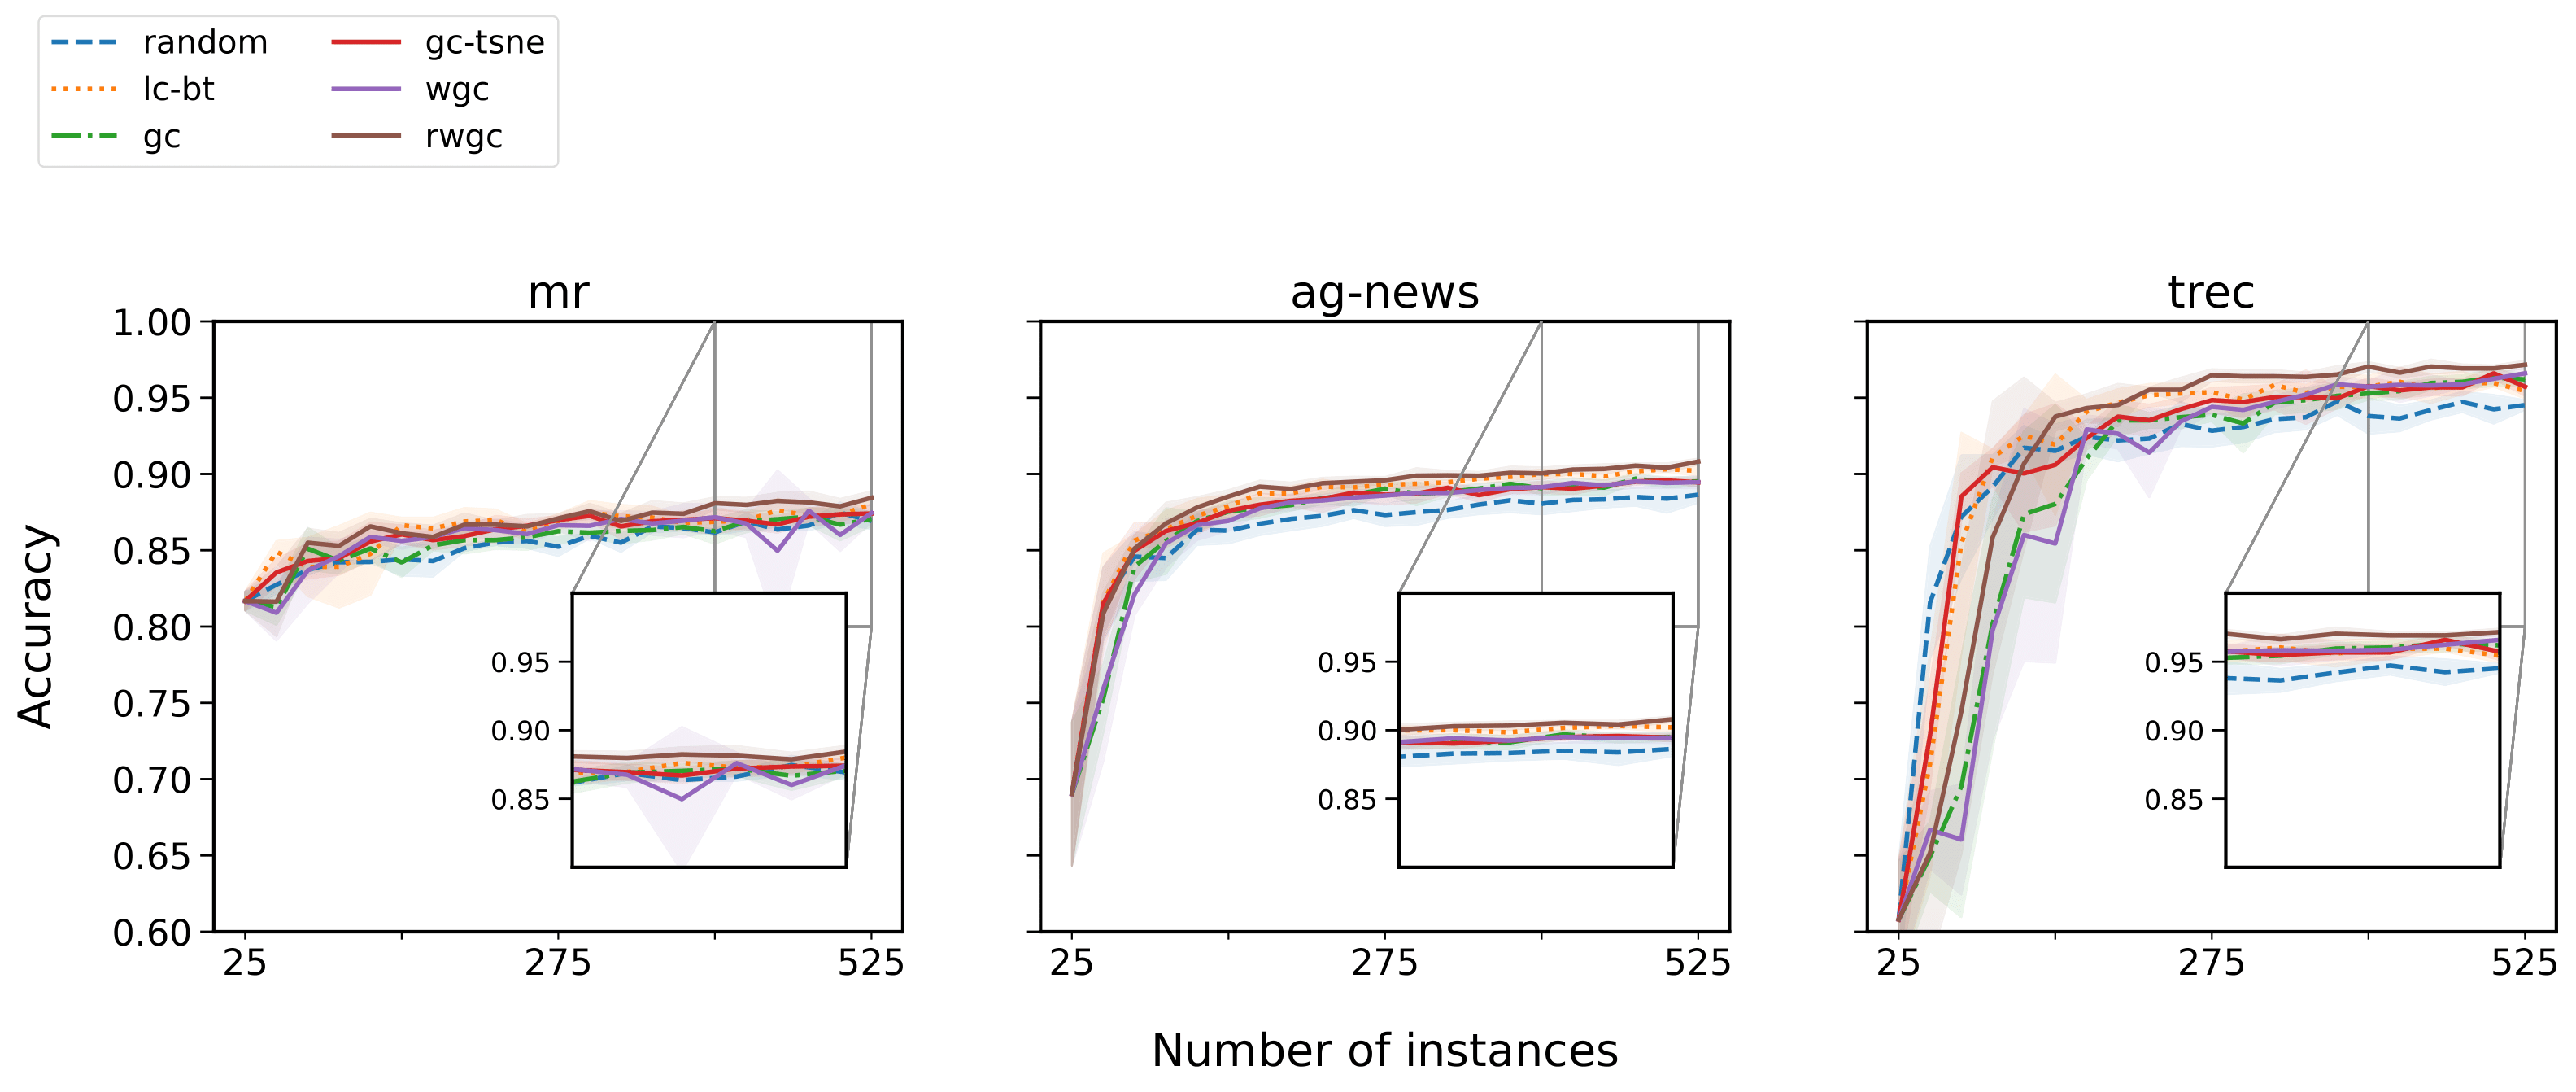
\includegraphics[width=1\textwidth,trim={0 0 0 4.83cm},clip]{img/setfit-plots-1.png}
    \caption{Active Learning curves of BERT (top row) and SetFit (bottom row) on each dataset when combined with eight query strategies: Random Sampling, Breaking-Ties, Core-Set, Core-Set with t-SNE, Core-Set with UMAP, Weighted Core-Set, Re-ranked Core-Set and Class-Balanced Core-Set. The lines represent the mean accuracy, and the surrounding bounds represent the standard deviation over five runs.}
    \label{fig:learning-curves}
\end{figure}

% GENERAL: Comparing models
Overall, the SetFit learning curves generally outperform the BERT model and seem to show much less variation between the different query strategies (Figure~\ref{fig:learning-curves}). This is reflected not only in the mean curve progressions of each model, but also in the smaller standard deviations of each individual strategy. Even in the case of BERT's resulting AL curves, the most noticeable accuracy differences seem to mainly occur in early iterations. Generally, the mean accuracy scores of the different strategies tend to lie in a similar range by the final iteration. 

I first compare and contrast the different results for the training of the BERT model (Figure~\ref{fig:learning-curves}, top row). We can clearly see general upward trends to varying degrees, depending on the dataset. The highest final accuracies are achieved on the TREC dataset, whereas the learning curves for AGN have the fastest increase in early iterations. Both seem to resemble a saturation curve, with TREC's mean accuracy values starting to slowly level out around 90\%, while AGN's stop around 85\% near the second half of the learning process. From this point on, the curves of both datasets gradually rise by around 5 percentage points towards the end of training. In contrast to this, the learning curves on MR show a more gradual, steady rise throughout the entire process and finish with slightly lower overall accuracies, with all strategies coming out to just under or around 80\%. 

% BERT: comparing query strategies
When comparing the curves of the different query strategies, we can see that, specifically in the case of BERT, CS does indeed seem to underperform when compared to the baseline approaches. This is mainly noticeable when looking at the earlier iterations (between queries 1 and 10). The underperformance of CS becomes even more apparent when considering the fact that the learning curves of RS are consistently above those of CS. This further reinforces the impression that Core-Set may have weaknesses within the domain of text classification. 

In the case of AGN and TREC, we can clearly see BT achieve high performances throughout, although CS--tSNE is able to compete very closely on AGN. Interestingly enough, RS has managed to achieve similar scores to the strategies mentioned previously in these cases.

We also observe that, in most cases, the different variations of Core-Set seem to be on par with or more performant than the original Core-Set. Both dimensionality reduction-based approaches, especially CS--tSNE, look to be strong contenders in most cases and manage to perform similarly to or better than CS and the remaining variants. 

CS--UMAP performs favorably, especially in the case of MR, where it remains on the upper end of accuracy scores throughout and manages to outperform all other strategies by the final iteration. In the case of AGN and TREC, we still find improvements to Core-Set during training, although these datasets seem to generally favor the t-SNE approach. Interestingly, the learning curve of CS--UMAP takes a dip in the latter half of training on the TREC dataset and rises rapidly again in the final iterations. Notably, a comparable sharp decrease is apparent in the first half of training on the same dataset for CS--tSNE's curve.

The class-balanced approach, on the other hand, does not seem to show significant accuracy improvements during training in comparison to CS. One discernible difference with the learning curve of CB--CS is noticeable on the MR dataset, where its curve seems to have much fewer fluctuations than CS and its other variations. Generally, however, CS and its class-balanced version show very similar learning curve trends across all three datasets. 

Weighted Core-Set and Re-ranked Core-Set are in a similar vein to, albeit oftentimes slightly above, the class-balanced approach. Both curves fluctuate around the same level or slightly higher than CS, but do not manage to surpass the baseline approaches in early iterations. We can see that in the case of AGN, the re-ranked strategy's learning curve even takes a dip in mean accuracy towards the end, resulting in a mean final accuracy below that of all other strategies by the final iteration despite being relatively competitive in prior iterations.

% SetFit: comparing datasets
The SetFit learning curves (Figure~\ref{fig:learning-curves}, bottom row) show much less fluctuation throughout the individual learning curves, as well as smaller discrepancies between the different query strategies during training. 

In the case of MR, all strategies have very similar accuracy curves and bundle tightly around the final iterations, with all final values somewhere around 87.5\%. For this dataset, the increase throughout the entire process is very minimal, amounting to only around 5 percentage points from the first query to the end of training. As for AGN and TREC, more learning progress is visible from beginning to end. Moreover, the margins between the curves are slightly wider, and some differences can be noted when comparing the different strategies. For these two datasets, the curves again show large early increases around the first five iterations, with the values starting to level out somewhere between instance 150 and 275. For these datasets, the values by the last iteration are also higher than for MR, with final results around the 90\% mark on AGN and around 95\% on TREC.

% SetFit: comparing query strategies
Again, BT stands out as one of the best strategies, with CS--tSNE generally following a similar trend. In contrast to BERT, CS itself does not seem to underperform in any considerable way. Only in the first half of the learning process on TREC can we see some kind of discernible difference between CS and the other curves. In these earlier instances, CS is outperformed by the baseline strategies as well as the dimensionality reduction-based strategies. 

In this diagram, we can also observe that the different strategies fall into two ``groups'' of curve progressions in the beginning iterations. Similarly to BERT's learning curves, we can see WCS, RCS and CB--CS following a very close trend to that of CS. The other query strategies (RS, BT, CS--tSNE, CS--UMAP) seem to follow a slightly higher, but similarly bundled, trend. This clustering of query strategies is only noticeable on the TREC dataset curves, whereas the other graphs seem to show all or most strategies bundled closer together overall.

One slight outlier in these graphs is RS, of which the accuracy values stay slightly below the other query strategies in the second half of each run, specifically when considering AGN and TREC. For these two datasets, RS seems to be competitive in early iterations, outperforming CS and many of the other strategies, but progress rapidly slows, resulting in lower final scores than the other strategies.

%The following page shows two tables containing the mean accuracy (Table~\ref{table-results-acc}) and mean AUC values (Table~\ref{table-results-auc}) corresponding to the learning curves. 

\clearpage \newpage

% NEW TABLES
\begin{sidewaystable}[htpb]

\centering
\fontsize{8pt}{9pt}\selectfont%
\renewcommand{\tabcolsep}{6pt}%
\begin{tabular}{@{}ll@{\hspace{10pt}} r @{${}\pm{}$} r r @{${}\pm{}$} r r @{${}\pm{}$} r r @{${}\pm{}$} r r @{${}\pm{}$} r r @{${}\pm{}$} r r @{${}\pm{}$} r r @{${}\pm{}$}r @{}}
\toprule
\textbf{Dataset} & \textbf{Model} & \multicolumn{14}{c}{\textbf{Query Strategy}}\\
\cmidrule{3-18} & & \multicolumn{2}{c}{\hspace*{-6pt}RS} & \multicolumn{2}{c}{BT} & \multicolumn{2}{c}{CS} & \multicolumn{2}{c}{\hspace*{4pt}CS--tSNE} & \multicolumn{2}{c}{\hspace*{4pt}CS--UMAP} & \multicolumn{2}{c}{\hspace*{4pt}WCS} & \multicolumn{2}{c}{\hspace*{4pt}RCS} & \multicolumn{2}{c}{\hspace*{4pt}CB--CS} \\
\midrule

\multirow{2}{*}{AGN}  & BERT & 0.884 & 0.004 &  \bfseries 0.889 & \bfseries 0.010 & 0.874 & 0.012 & 0.881 & 0.010 & 0.884 & 0.010 & 0.873 & 0.011 & 0.785 & 0.221 & 0.866 & 0.016\\ 
 & SetFit & 0.886 & 0.006 & \bfseries 0.902 & \bfseries 0.004 & 0.895 & 0.003 & 0.895 & 0.003 & 0.899 & 0.001 & 0.895 & 0.005 & 0.895 & 0.004 & 0.898 & 0.006 \\

\midrule

\multirow{2}{*}{MR}  & BERT & 0.806 & 0.011 & 0.815 & 0.009 & 0.770 & 0.015 & 0.796 & 0.020 & \bfseries 0.819 & \bfseries 0.011 & 0.806 & 0.014 & 0.811 & 0.013 & 0.793 & 0.021\\ 
 & SetFit & 0.869 & 0.006 & \bfseries 0.880 & \bfseries 0.005 & 0.871 & 0.005 & 0.874 & 0.005 & 0.876 & 0.008 & 0.874 & 0.007 & 0.870 & 0.004 & 0.870 & 0.006 \\

\midrule 

\multirow{2}{*}{TREC}  & BERT & 0.904 & 0.018 & \bfseries 0.920 & \bfseries 0.014 & 0.902 & 0.021 & 0.912 & 0.009 & 0.898 & 0.033 & 0.897 & 0.027 & 0.897 & 0.036 & 0.872 & 0.048\\ 
 & SetFit & 0.945 & 0.004 & 0.954 & 0.006 & 0.962 & 0.004 & 0.957 & 0.007 & 0.962 & 0.010 & \bfseries 0.966 & \bfseries 0.004 & 0.962 & 0.003 & 0.956 & 0.007 \\

\bottomrule
\end{tabular}

\caption{%
Final accuracy per dataset, model, and query strategy. We report the mean and standard deviation over five runs. The best result per dataset is printed in bold.}
\label{table-results-acc}

\vspace{2\baselineskip}

\centering
\fontsize{8pt}{9pt}\selectfont%
\renewcommand{\tabcolsep}{6pt}%
\begin{tabular}{@{}ll@{\hspace{10pt}} r @{${}\pm{}$} r r @{${}\pm{}$} r r @{${}\pm{}$} r r @{${}\pm{}$} r r @{${}\pm{}$} r r @{${}\pm{}$} r r @{${}\pm{}$} r r @{${}\pm{}$} r @{}}
\toprule
\textbf{Dataset} & \textbf{Model} & \multicolumn{14}{c}{\textbf{Query Strategy}}\\
\cmidrule{3-18} & & \multicolumn{2}{c}{\hspace*{-6pt}RS} & \multicolumn{2}{c}{BT} & \multicolumn{2}{c}{CS} & \multicolumn{2}{c}{\hspace*{4pt}CS--tSNE} & \multicolumn{2}{c}{\hspace*{4pt}CS--UMAP} & \multicolumn{2}{c}{\hspace*{4pt}WCS} & \multicolumn{2}{c}{\hspace*{4pt}RCS} & \multicolumn{2}{c}{\hspace*{4pt}CB--CS}\\
\midrule
 
\multirow{2}{*}{AGN}  & BERT & 0.790 & 0.015 & \bfseries 0.800 & \bfseries 0.009 & 0.735 & 0.020 & 0.792 & 0.007 & 0.772 & 0.019 & 0.731 & 0.014 & 0.741 & 0.015 & 0.733 & 0.017\\ 
 & SetFit & 0.865 & 0.007 & \bfseries 0.881 & \bfseries 0.004 & 0.871 & 0.005 & 0.875 & 0.004 & 0.879 & 0.004 & 0.870 & 0.003 & 0.870 & 0.002 & 0.873 & 0.003 \\

\midrule

\multirow{2}{*}{MR}  & BERT & \bfseries 0.750 & \bfseries 0.007 & 0.746 & 0.011 & 0.718 & 0.009 & 0.741 & 0.017 & 0.748 & 0.005 & 0.720 & 0.004 & 0.718 & 0.005 & 0.706 & 0.015\\ 
 & SetFit & 0.854 & 0.002 & 0.864 & 0.005 & 0.856 & 0.003 & 0.862 & 0.003 & \bfseries 0.866 & \bfseries 0.005 & 0.858 & 0.007 & 0.857 & 0.003 & 0.859 & 0.002 \\

 \midrule
 
\multirow{2}{*}{TREC}  & BERT & 0.674 & 0.029 & \bfseries 0.709 & \bfseries 0.008 & 0.594 & 0.022 & 0.676 & 0.037 & 0.609 & 0.029 & 0.629 & 0.024 & 0.624 & 0.012 & 0.598 & 0.025\\ 
 & SetFit & 0.914 & 0.011 & \bfseries 0.923 & \bfseries 0.007 & 0.896 & 0.015 & 0.919 & 0.005 & 0.921 & 0.008 & 0.893 & 0.012 & 0.897 & 0.012 & 0.905 & 0.010 \\

 
\bottomrule
\end{tabular}

\caption{Final AUC per dataset, model, and query strategy. We report the mean and standard deviation over five runs. The best result per dataset is printed in bold.}
\label{table-results-auc}

\end{sidewaystable}

\clearpage

% Accuracy Table

%In Table~\ref{table-results-acc}, I show the reported mean final accuracy across all runs, as well as the standard deviation for each combination of dataset, model and query strategy. 

%Overall, Breaking-Ties dominates for almost every dataset on both models. Only for SetFit does another strategy achieve the highest overall final mean accuracy. Furthermore, we can see that RS outperforms CS when used with BERT throughout all datasets.

\subsection*{Tables}

In Table~\ref{table-results-acc}, BT dominates for almost every dataset on both models. Only in two cases does another strategy achieve the highest overall final mean accuracy. Even though the differences are predominantly characterized by very small margins throughout, there are still noteworthy observations to be made.

First, we can again see that RS outperforms CS when used with BERT across all datasets. CS seems to encounter minor difficulties, specifically on the MR dataset with BERT, where it marks the lowest result of all the strategies. Despite this, CS' training with the SetFit model yields improved results, particularly when contrasted with those achieved by RS with SetFit.

The results of the CS variations show small improvements in accuracy at various points. CS--tSNE and CS--UMAP most notably show slightly higher scores than CS in almost all cases. For CS--tSNE, the only exception is on TREC with SetFit. This row of results has some other noteworthy differences between query strategies. We can see that this is the only combination of model and dataset for which CS, along with all of its variations, scores a higher result than BT. In the case of CS--UMAP, the only instance where we find no improvement to CS is on the TREC dataset. However, we observe quite consistent accuracy scores above 80\% for this strategy across the board. Additionally, this approach manages to improve upon Core-Sets relatively low accuracy score on the MR dataset with BERT, increasing from 77\% to nearly 82\%.

Although WCS does have the best result in the case of the TREC dataset with SetFit, the remaining results in its column do not show consistent improvements when compared to CS. A similar sentiment applies to RCS and CB--CS, which show varied results in comparison to CS. The former method demonstrates a noticeable decrease to CS of around 9 percentage points for SetFit and AGN.

Even so, all of the CS variations also show some kind of improvement in the case of MR with BERT, in which CS has the lowest overall accuracy. Notably, AGN is the only dataset where CS--tSNE, WCS and RCS do not have any impact on the mean accuracy score in the case of SetFit. Even in cases where results are not exactly the same, they often remain within a one-standard-deviation range of each other. One row where this is most evident is the combination of SetFit and MR across all query strategies. In this row, we see even BT not achieve much improvement over the rest of the strategies. Especially the differences between RS and all CS-based approaches are negligible in this row. Generally, the SetFit results in all rows exhibit the smallest discrepancies, as is reflected in the learning curves presented previously.

% AUC Table: Models / Datasets
In the comparison of AUC values and variabilities for each combination of dataset, model, and query strategy (Table~\ref{table-results-auc}), SetFit again exhibits higher values than BERT overall, with considerably high results on the TREC dataset around the 90\% mark. The discrepancy between the two models is also most apparent for this dataset, with margins of 30\% or more in some instances. 

Regarding the other datasets, we again see MR with most of the lowest values overall, however, AGN's results generally seem to fall within a similar range. For both of these datasets, we can also see that the margins between the two models' performances are not nearly as evident as with TREC.

% AUC Table: query strategies
The top performing AUC results, similarly to the accuracy table, show BT as having the best results in almost all cases. Notably, RS manages to reach the highest AUC among all query strategies in the case of MR with BERT. For BERT, we observe even more noticeable discrepancies to CS across the board than in the accuracy tables. Additionally, the UMAP approach ranks highest in the case of MR with the SetFit model. However, both of these ranks are by relatively small margins compared to the rest of the results, especially the latter scenario. 

Again, the CS variations offer some minor improvements in multiple cases. Here, the similarities between the learning curves of CS, WCS, RCS and CB--CS become even more apparent, as the values of these strategies are almost equal in most instances. Nonetheless, the two dimensionality reduction approaches show higher AUC values than CS throughout. The largest improvement for CS--tSNE was achieved with BERT, namely on TREC (8.2 percentage points), with the second largest being on AGN (5.7 percentage points). The improvements with CS--UMAP are even more minor, mainly noticeable with BERT on AGN (3.7 percentage points) and MR (3 percentage points). 

\chapter{Discussion}

% INTRODUCTION
Although none of the proposed Core-Set variations manage to get scores consistently as high as the Breaking-Ties approach, we can still gather interesting insights from the conducted experiment. 

% ANSWERING RESEARCH QUESTIONS?
One presumption prior to the conducting of the experiment was that Core-Set may have mixed results in cases of text classification. Not only that, but according to \cite{DBLP:conf/kdd/0002MM21}, Core-Set's results with BERT sometimes lie even below the performances of Random Sampling. This experiment's results further support this statement, with Core-Set being outperformed by Random Sampling with BERT, both in mean accuracy and mean AUC.

In order to discuss the research questions posed in Chapter 1, I have structured the rest of this chapter according to the results of each approach presented in Chapter 3. Pertaining to the third research question, I have also conducted further analysis of the experiment results in order to determine whether the approach did indeed result in a more balanced distribution of classes in the labeled pool.

\section{Dimensionality Reduction-Based Approach}

The previously presented experiment has offered further insights with regard to the first research question. The first modification to Core-Set, which used t-SNE to reduce the dimensionality of word embeddings prior to the selection with $k$-Center greedy, generally managed to improve Core-Set over the three given datasets. Though the differences in the case of SetFit were very minor, we can observe more noticeable improvements in efficiency (i.e., mean AUC results) with BERT, where Core-Set seemed to have its weaknesses originally. The second technique used for this approach (UMAP) resulted in similar improvements to the Core-Set approach, which were most noticeable on the MR dataset with BERT. Again, the overall accuracy and AUC differences were minor in most instances, but overall positive nonetheless.

Between the two dimensionality reduction-based approaches, the differences observed were even more minor. Based on the experiment results, it is not yet clear which dimension is optimal for the reduced space, as the reduction to both two and 256 dimensions led to similarly positive outcomes. Furthermore, the optimal dimension may also depend on the underlying dataset. Due to this, it is also unclear which of the two techniques is superior for this particular task; to determine this, the techniques should be compared on the same reduction dimensions. In the case of t-SNE, this was not possible for higher dimensions due to the implementation limitations stated in Section 2.4. 

The demonstrated improvements of Core-Set with dimensionality-reduced embeddings may further support the impression that Core-Set encounters difficulties when faced with the task of higher-dimensional feature spaces \citep{DBLP:conf/iccv/SinhaED19}, as was also mentioned in Chapter 1. However, the exact impact of the degree to which the dimension is reduced (i.e., what dimensions Core-Set operates most optimally on) still remains unclear. Additionally, these techniques inevitably lead to longer runtimes, especially in the case of the lesser-optimized t-SNE. In the context of this thesis' experiment, this factor did not lead to any major issues or difficulties; however, in the case of larger datasets or larger feature spaces, this approach may lead to considerable runtime increases. In these cases, understanding the tradeoff between performance boosts and longer runtimes becomes increasingly important. 

\section{Uncertainty-Based Approach}

With respect to the second research question, I presented and implemented two uncertainty-based approaches.  
Both attempts have shown minor, but generally negligible improvements, with certain cases even showing slight drops in performance. 

Though WCS and RCS had generally similar results overall, they still lean slightly in favor of WCS due to the improvements on TREC with SetFit and AGN with BERT, in which RCS fell short. Another aspect outside of performance that may favor WCS over RCS is the ease of implementation and interpretability, which are more straightforward for the weighted approach. In addition, WCS does not perform what are essentially two instance selection runs per query, which is the case in the re-ranked approach and might lead to slightly longer runtimes. 

It may be that the combinations of Core-Set with the uncertainty-based approaches attempted here were simply too minor to have a noticeable impact on the resulting accuracy scores. In the case of WCS, the linear combination may place an overwhelming emphasis on Core-Set, leading to results that do not differ much from the original $k$-Center algorithm. In the case of RCS, it may similarly be the case that re-ranking only $2b$ instances is not sufficient for performance changes, which might explain why this approach also does not manage to outperform either of the approaches it is based on.

With these mixed results in mind, my conclusion regarding this research question is negative.

\section{Class Balance-Based Approach}

Finally, with regard to the third research question, it is apparent that the proposed class balance-based approach does not manage to improve upon Core-Set's performance. The accuracy and AUC values are, in most cases, either on par with or slightly below those of Core-Set. This is also reflected in the learning curves, where no clear improvement to Core-Set is visible throughout. In the case of MR, one might initially assume little to no impact for class balancing due to the fact that this dataset only has two classes and, as a consequence, already has relatively balanced class distributions regardless. However, the experiment also considered AGN and TREC, two multi-class datasets, which showed similarly unchanged performances. So, the class balancing employed for this approach did not seem to improve Core-Set, even in the case of multi-class datasets.

\begin{figure}[htbp]
    \centering
    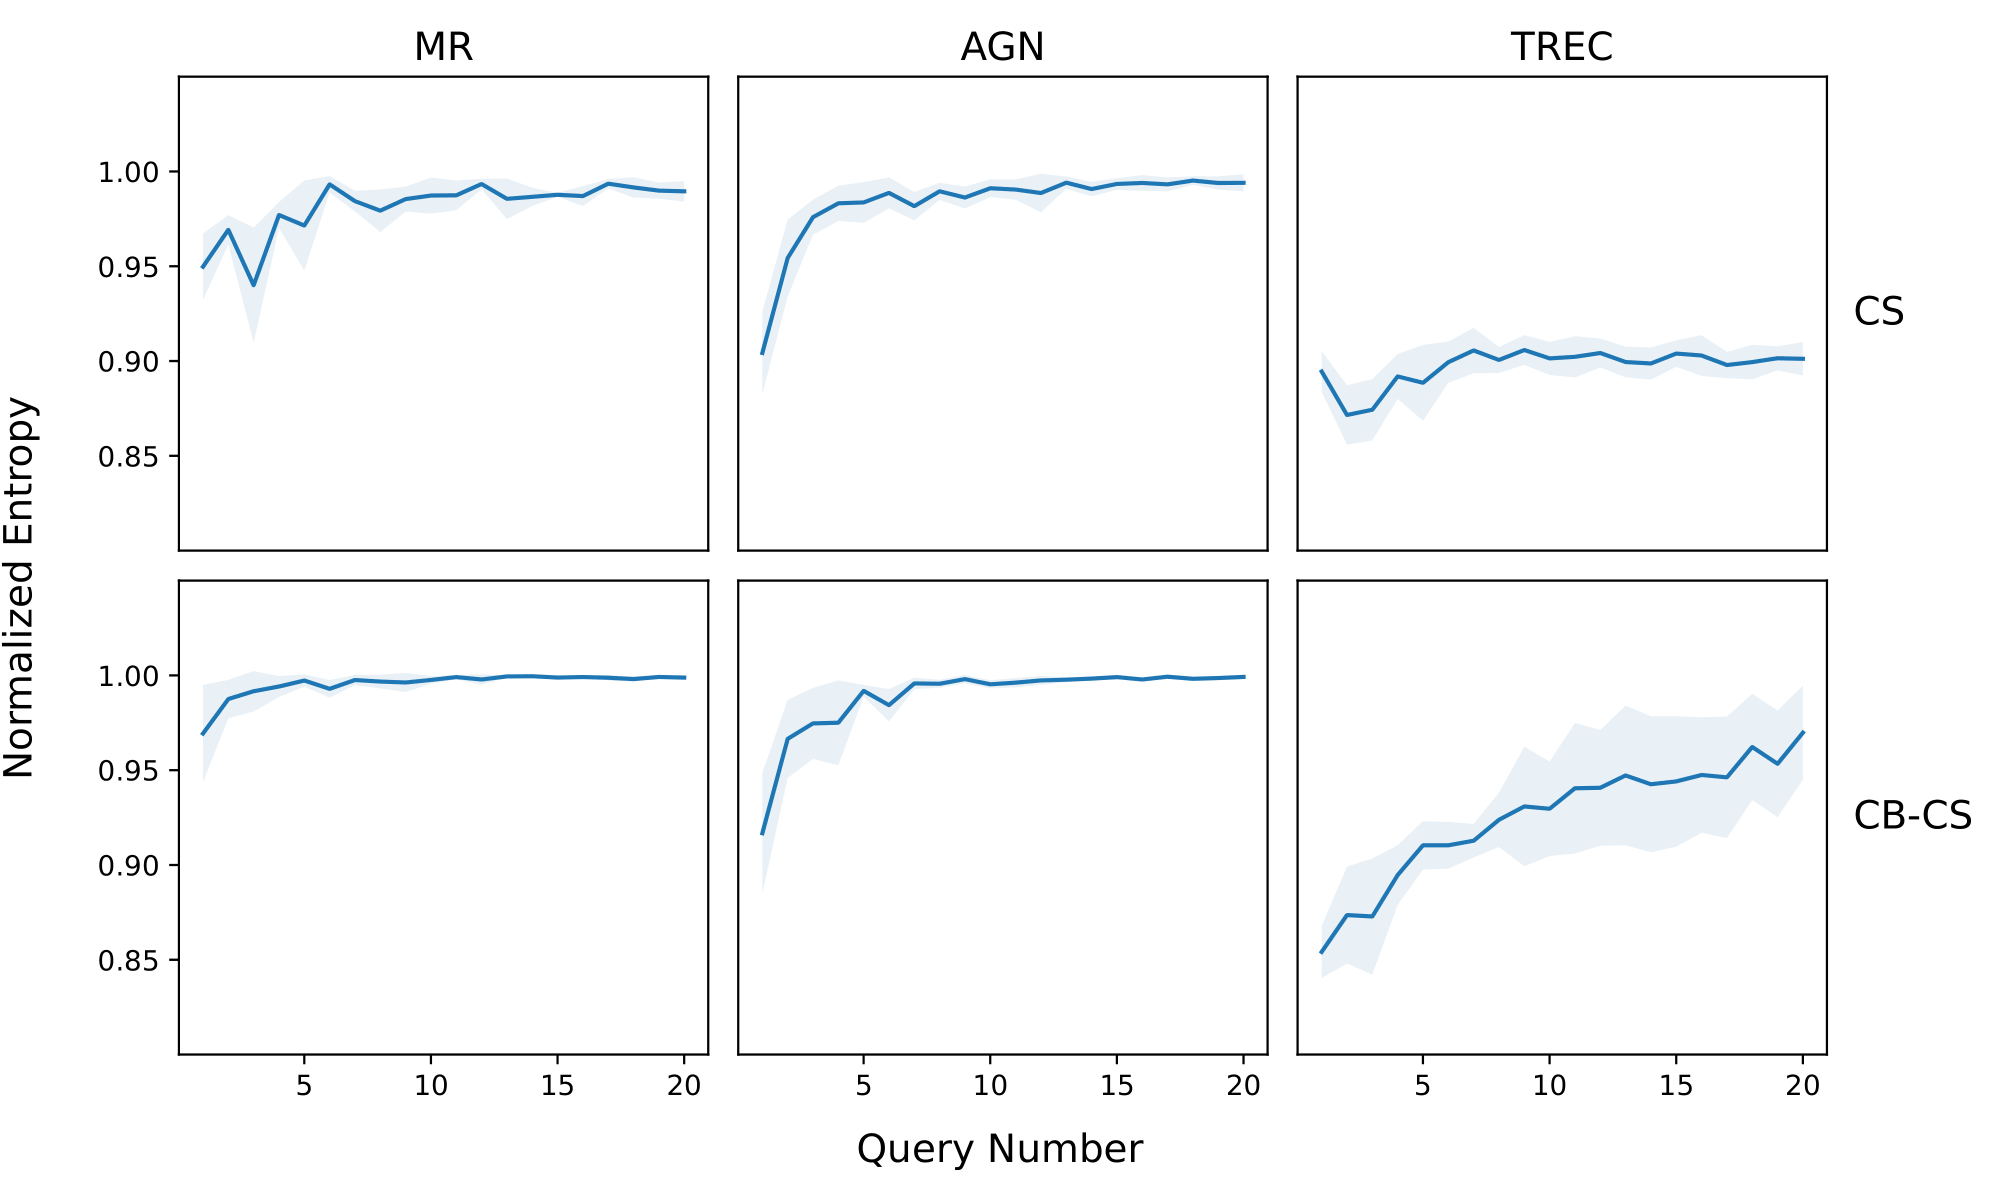
\includegraphics[scale=0.55]{img/entropy_plots_new-1.png}
    \caption{Normalized entropy curves for instances selected during AL with BERT using Core-Set and Class-Balanced Core-Set. The lines represent the mean accuracy, and the surrounding tubes represent the standard deviation over five runs.}
    \label{fig:entropy-plot}
\end{figure}

In order to investigate the functionality of the class-balanced approach, I tracked the class distributions after each query of the previously conducted experiment. As a result, I was able to observe an overall positive impact of the balancing on the class distribution within the labeled pool. This impact was measured using the normalized entropy within the labeled pool after each iteration, as explained in Chapter 3. Similar to the learning curves in Section 4.3, I have plotted the mean over five runs in Figure~\ref{fig:entropy-plot}. 

% OLD ENTROPY PLOT
\iffalse
\begin{figure}[htbp]
    \centering
    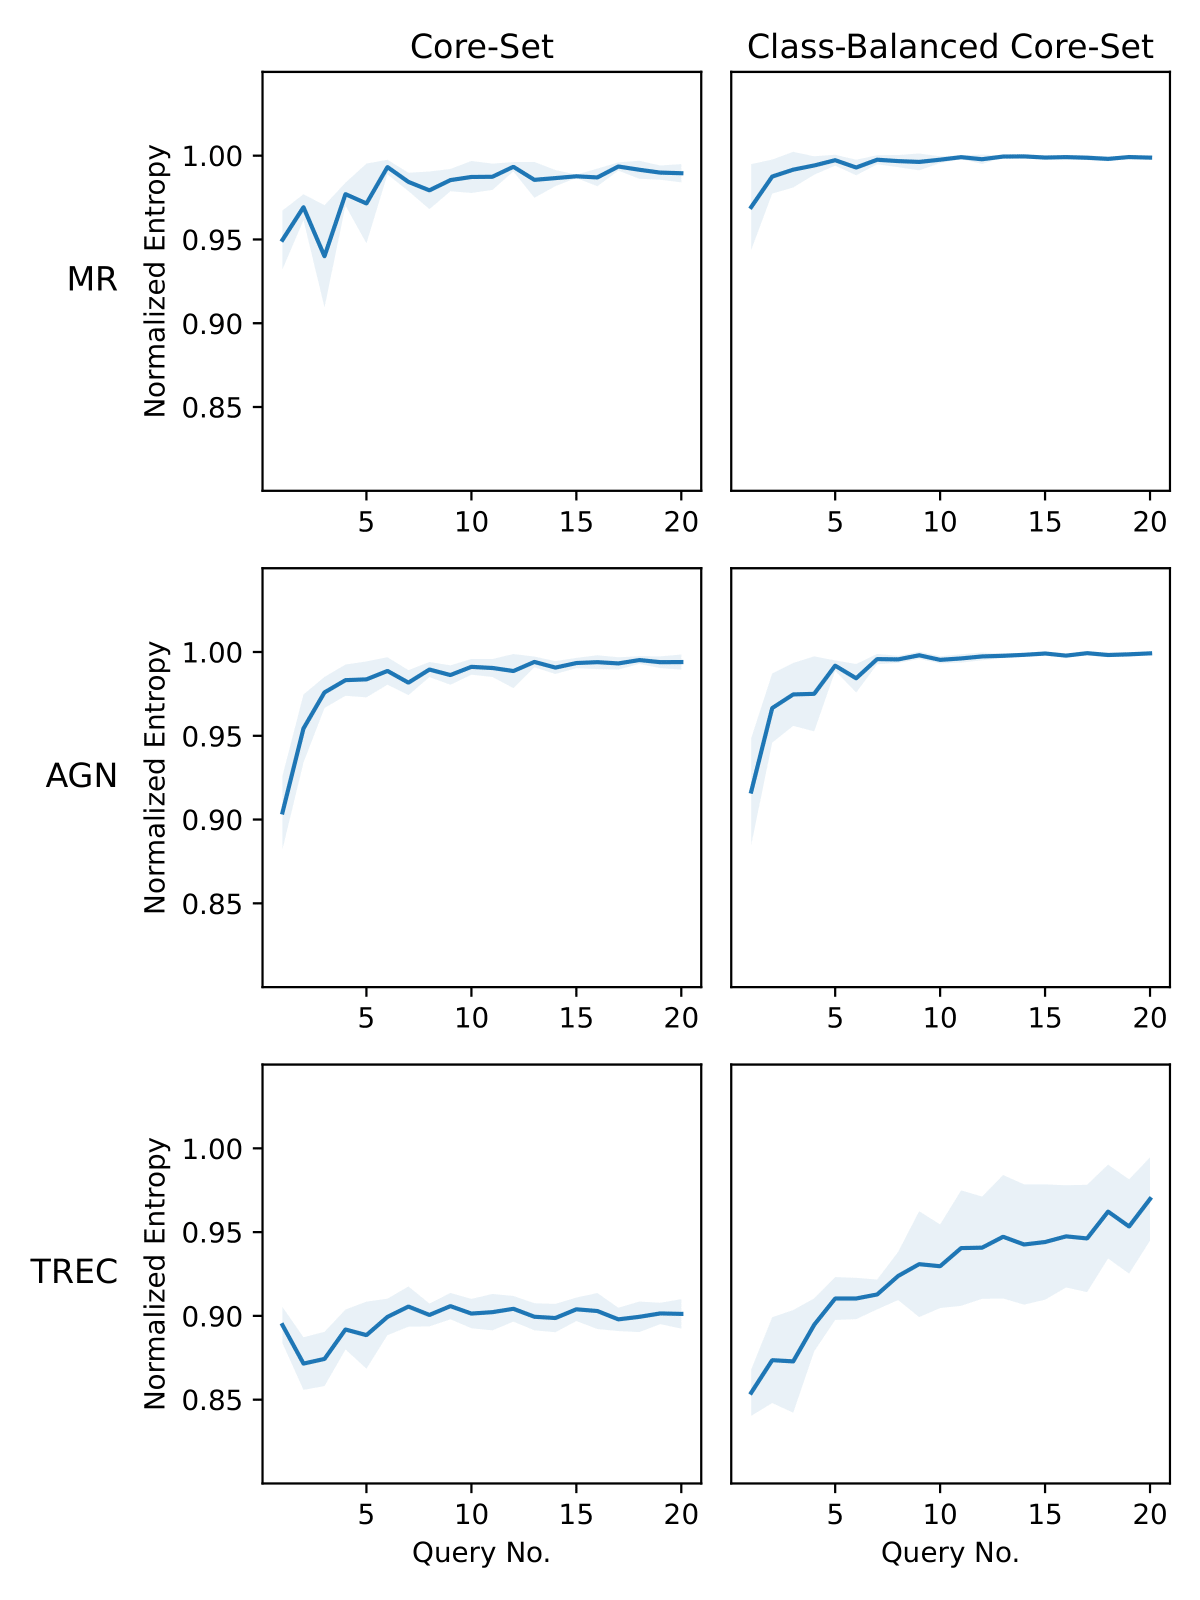
\includegraphics[scale=0.6]{img/entropy_plots-1.png}
    \caption{Normalized entropy curves for instances selected during AL with BERT using Core-Set and Class-Balanced Core-Set. The lines represent the mean accuracy, and the surrounding tubes represent the standard deviation over five runs.}
    \label{fig:entropy-plot}
\end{figure}
\fi

We can see that for both strategies, the normalized entropy generally increases or stays relatively constant with each query. In the case of MR, we observe only minor changes in the class distribution throughout the learning process. This may be in part attributed to the fact that this dataset only has two classes that are distributed evenly. Nonetheless, we observe the class-balanced approach to have a more stable mean normalized entropy in the first half of the learning process, whereas the regular Core-Set selection has slight fluctuations. Nevertheless, both curves run somewhere within the range of 0.95 and 1, indicating a very close to even distribution in both cases. 

For AGN, the difference between Core-Set and the class-balanced approach seems to be even less evident. In both cases, we observe a saturation curve beginning around 0.9 and evening out close to 1 around the fifth query. Although AGN has twice as many classes as MR, it is also a class balanced dataset with equal amounts of instances from each class, which may explain the depicted results.

The dataset in which a change in class distribution within the labeled pool is most distinct is TREC. Here, we note a relatively constant curve around or below a normalized entropy of 0.9 in the case of Core-Set, whereas the class-balanced approach manages to select an increasingly even distribution. In this case, the normalized entropy gradually rises from roughly 0.85 to around 0.97. Still, the standard deviation increases in later iterations, becoming clearly higher than in all other cases. 

One reason for these differences in the efficacy of the class-balanced approach is the underlying class distribution of each dataset. In the case of MR and AGN, we have uniform distributions across all classes, whereas TREC is an inherently class-imbalanced dataset.\footnote{The six classes are distributed as follows: 'ENTY' (22.9\%), 'HUM', (22.4\%), 'DESC' (21.3\%), 'NUM' (16.4\%), 'LOC' (15.3\%), 'ABBR' (1.6\%) \citep{DBLP:journals/nle/LiR06}.} Consequently, the class-balanced approach has very little impact on the distributions of the selected instances, which are nearly uniformly distributed in the first place. TREC, in contrast, has slightly imbalanced classes, resulting in the possibility for improvement using the class-balanced approach. I conclude that the balancing of classes within the Core-Set selection has been achieved, though this has not been shown to lead to improved performances in this case.

\section{Limitations}

Naturally, there are some limitations to consider with this experiment. On one hand, the training data used only encompassed three different datasets. These datasets do attempt to cover a variety of purposes, class cardinalities, and sizes, but in order to further verify the effectiveness of the proposed approaches, more datasets should be used. 

Another aspect that was not considered by my experiment is the effect of each approach on the respective runtime. This may be especially relevant when considering a dimensionality reduction algorithm such as t-SNE, which could have a significant impact when training on larger datasets. 

Furthermore, this experiment's result evaluation only took into account the respective accuracy and AUC metrics. For the purpose of evaluating the results of each strategy, it may be worth considering other commonly used metrics, such as the $\text{F}_1$-score. Even so, this metric attributes equal importance to precision and recall, of which the relative importance is often highly dependent on the specific application \citep{DBLP:journals/sac/HandC18}.

Finally, it is worth underlining the fact that this thesis examined Core-Set as the basic $k$-Center greedy approach, whereas \cite{DBLP:conf/iclr/SenerS18} propose a slightly optimized, robust $k$-Center approach that minimizes outliers. This approach was not used for implementation reasons, as the solution for robust $k$-Center's feasibility check depends on Gurobi \citep{gurobi}, a proprietary optimization framework. As a result, the results of Core-Set and the corresponding modifications used in this experiment may not be optimal.

\section{Future Research}

As mentioned earlier, this experiment was conducted on three datasets, two of which have uniform class distributions. With regard to the class-balanced approach, it may be worth examining the effect on various datasets with more imbalanced class distributions. Not only may this result in more significant improvements to the normalized entropy, but possibly a more noticeable impact on the learning process itself. 

Regarding the dimensionality reduction-based approaches, it may be worth examining the effect of reducing to different dimensions, as well as potentially tuning some of the many hyperparameters. In the case of UMAP for instance, it may be worth examining the effect of reducing to 128, 64, 32 dimensions, or even less. For t-SNE, hyperparameters such as perplexity, which loosely describes the balance of attention between local and global structures, may also have a significant impact on the technique's results \citep{wattenberg2016how}. 

Concerning the two uncertainty-based approaches, it may be worth looking into the effect of a different Core-Set to Breaking-Ties ratio for the weighted linear combination in WCS (80--20) or modifying the number of instances to re-rank in RCS ($2b$). 

Furthermore, it could be worth investigating the effect of combining two or more of the approaches presented here. If two strategies such as CS--tSNE and CB--CS only offer minor improvements in some cases, maybe a combination of the two approaches could contribute to more efficient learning. Similarly to \cite{DBLP:journals/corr/abs-2110-03785}, the combination of these approaches would be motivated by the idea of creating a new strategy that potentially makes use of the positive aspects of each method. 

Of course, some of the aspects mentioned in the previous section could be added to this experiment for further research. Examining other metrics such as the $\text{F}_1$-score (while taking into account its potential caveats) and total runtimes, as well as considering other models and datasets, may offer additional insights in determining the utility of the presented approaches. 

\chapter{Conclusion}

In this thesis, I examined the effect of Core-Set as an AL query strategy for text classification tasks, pointed out its inherent limitations, and explored possibilities for improving the approach. To this end, I created an AL experiment in which I compared Core-Set with five variations and two baseline approaches using two models across three different datasets. The motivation for doing this was to see if Core-Set does indeed achieve mixed results within the field of text classification and to attempt to work toward a possible improvement in this regard. 

To address three possible limitations of Core-Set in the context of AL, I presented three categories of approaches (dimensionality reduction-based, uncertainty-based, class balance-based), which resulted in five different modifications to the original $k$-Center greedy algorithm. I implemented and tested the various strategies within an AL experiment setup using the datasets and models mentioned previously, and discussed their results using various metrics. 

The experiment's results show Core-Set producing mixed results in many cases when compared to the baseline strategies. This aligns with what was shown in \cite{DBLP:conf/kdd/0002MM21} and briefly mentioned in \cite{DBLP:conf/aaai/ColemanCKCBBNSZ22}. Moreover, the results conclude that we can observe some slight improvements of Core-Set's performances when used in conjunction with two nonlinear dimensionality reduction techniques, t-SNE and UMAP. These techniques were selected not only for the sake of variation but also to examine potential differences in results based on the dimensions of the embedding reductions. Furthermore, the uncertainty-based approach and the class balance-based approach do not seem to considerably impact Core-Set's results. The uncertainty-based approaches, based on a weighted and a re-ranking scheme, attempted to incorporate uncertainties from Breaking-Ties, another well-established query strategy, into the ``decision-making'' process of Core-Set. However, these approaches did not manage to achieve consistently higher results than Core-Set. Finally, the class balance-based approach attempted to create Core-Set selections with balanced class distributions with the intention of learning from instances with all kinds of class labels. Although this did not result in any significant performance changes, I was able to observe an overall positive impact on the class distributions of the labeled instance pools in the case where the dataset had imbalanced classes by measuring the respective normalized entropy values.

In general, the modifications to the Core-Set approach presented and discussed within this thesis have yielded similarly mixed experiment results overall. Although the overall performance of Breaking-Ties was not surpassed by any of the approaches, the two dimensionality reduction approaches were able to achieve minor improvements to Core-Set. Moreover, the difference between the two models, BERT and SetFit was demonstrated, with the latter outperforming the former on three text classification datasets. Overall, I was not able to determine which aspect of the different approaches was most conducive to the success of Core-Set. Despite relatively large differences in the reduced dimensions, the results do not largely favor one reduction space over the other. Similarly, I was unable to discern noticeable changes between the two uncertainty-based Core-Sets, despite their differing approaches.

Nonetheless, the insights gained do show some positive aspects and leave room for additional research and examination considering each strategy. With an ever-growing need for efficient text classification, improving state-of-the-art approaches to machine learning will continue to be an important endeavor.

% \chapter*{Acknowledgements} % optional
% I thank the authors of the webisthesis template for their excellent work!

% \listoffigures % optional, usually not needed

% \listoftables % optional, usually not needed

% \listofalgorithms % optional, usually not needed
%    requires package algorithm2e

% optional: list of symbols/notation (e.g., using the nomencl package) but usually not needed

%\include{chapter1}
%\include{chapter2}

%\include{appendixA}

% TODO: MAYBE GET RID OF THIS
\appendix
\chapter{Implementation Details}

The experiment setup is based on a pre-existing AL environment created with \cite{schroeder2023small-text}. This also includes the implementation of $k$-Center greedy as well as various methods concerning class redistributions. In addition, well-known machine learning libraries such as Scikit-Learn, HuggingFace, NumPy, and SciPy were used for the implementation of the query strategies, as well as for the calculation of the normalized entropies in Section 3.3. For the dimensionality reduction with UMAP, I used the \href{https://github.com/lmcinnes/umap}{umap-learn} library \citep{DBLP:journals/corr/abs-1802-03426}. The models that were fine-tuned within the experiment are \href{https://huggingface.co/google-bert/bert-base-uncased}{bert-base-uncased} and \href{https://huggingface.co/sentence-transformers/paraphrase-mpnet-base-v2}{
paraphrase-mpnet-base-v2}. The datasets were also obtained via the \href{https://github.com/huggingface/datasets}{huggingface datasets} library. All libraries mentioned were used within a Python 3.8 environment.

% Bibliography
\bibliographystyle{plainnat} % requires package natbib. An alternative is apalike
\bibliography{literature}    % load file literature.bib

\end{document}
